\documentclass{beamer}

% Load packages
\usepackage[utf8]{inputenc}
\usepackage[pdf]{graphviz}

% Look and feel
\usetheme{metropolis}

%% Add frame subtitle
%% https://tex.stackexchange.com/a/514348
\makeatletter
\setbeamercolor{framesubtitle}{fg=mDarkTeal}
\setbeamerfont{caption}{size=\scriptsize}
\defbeamertemplate*{frametitle}{myframetitle}{%
    \nointerlineskip
    \begin{beamercolorbox}[%
        wd=\paperwidth,%
        sep=0pt,%
        leftskip=\metropolis@frametitle@padding,
        rightskip=\metropolis@frametitle@padding,
        ]{frametitle}%
        \metropolis@frametitlestrut@start
        \quad\insertframetitle%%%%%%%%%%%%%%%%%%%%%%
        \nolinebreak
        \metropolis@frametitlestrut@end
    \end{beamercolorbox}\par
    \usebeamerfont{framesubtitle}%
    \usebeamercolor[fg]{framesubtitle}%
    \vskip3pt
    %\hspace*{-2.5\metropolis@frametitle@padding}%
    \insertframesubtitle
    \vskip3pt
}
\makeatother
\setbeamertemplate{frametitle}[myframetitle]

\usefonttheme[onlymath]{serif} % article style math

% 
\setlength{\abovedisplayskip}{-5pt}
\setlength{\belowdisplayskip}{-5pt}

% Title
\title[The RITAS algorithm]{The RITAS algorithm}
\subtitle{A constructive yield monitor data processing algorithm}
\author[Damiano, Niemi]{Luis Damiano}
\date{2020-10-21}
\institute[ISU]{Department of Statistics\\Iowa State University}

%%%%%%%%%%%%%%%%%%%%%%%%%%%%%%%%%%%%%%%%%%%%%%%%%%%%%%%%%%%%%%%%%%%%%%%%%%
% Document                                                               %
%%%%%%%%%%%%%%%%%%%%%%%%%%%%%%%%%%%%%%%%%%%%%%%%%%%%%%%%%%%%%%%%%%%%%%%%%%
\begin{document}

\begin{frame}
  \maketitle

  {\footnotesize
    Funded, in part, by
    \begin{itemize}
    \item[-] the Iowa State University Presidential Interdisciplinary
      Research Initiative on C-CHANGE: Science for a Changing Agriculture
    \item[-] Foundation for Food and Agriculture Research.
    \end{itemize}
  }
\end{frame}

\begin{frame}
  
  \frametitle{Road map}
  \tableofcontents
  
\end{frame}

%%%%%%%%%%%%%%%%%%%%%%%%%%%%%%%%%%%%%%%%%%%%%%%%%%%%%%%%%%%%%%%%%%%%%%%%%%
% Intro                                                                  %
%%%%%%%%%%%%%%%%%%%%%%%%%%%%%%%%%%%%%%%%%%%%%%%%%%%%%%%%%%%%%%%%%%%%%%%%%%

\section{Introduction}

\begin{frame}
  \frametitle{Context}

  % Worked on this first summer
  % The original STRIPS research question (link) needed a good way to
  % assign each observation to a treatment zone (show figure from
  % that report)
  
  \begin{figure}
    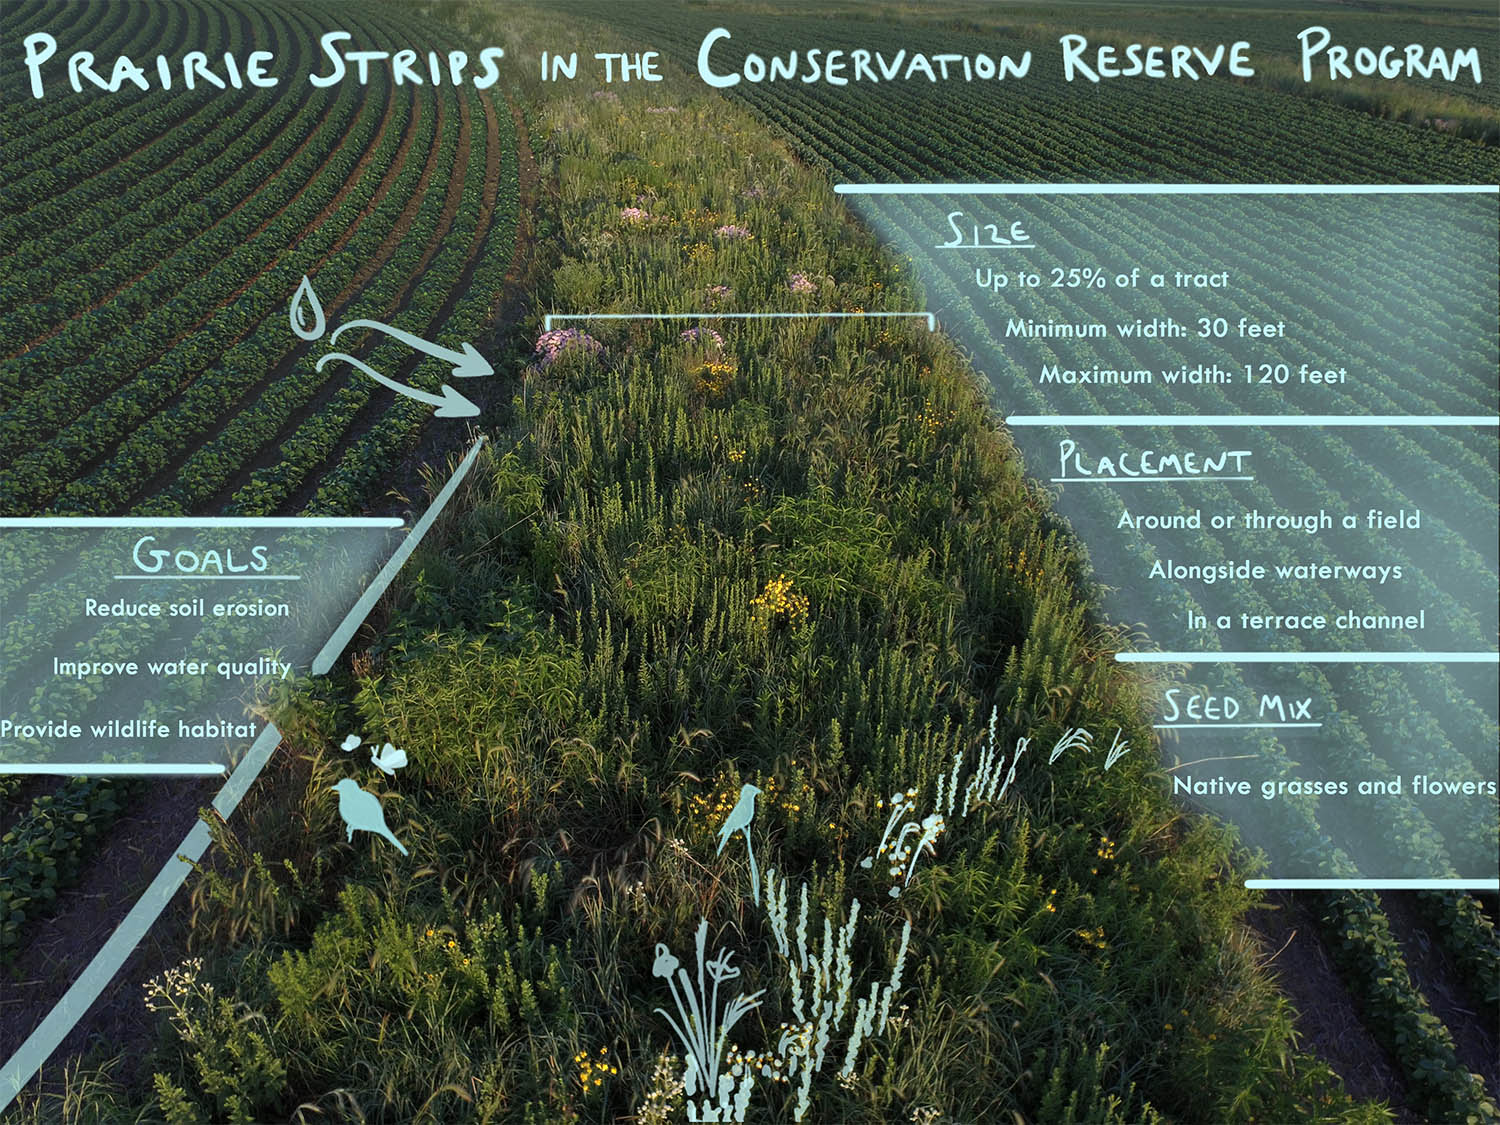
\includegraphics[width=0.95\textwidth]{./figures/strips_prairie.jpg}
  \end{figure}
    
\end{frame}

\begin{frame}
  \frametitle{Context}
  
  \begin{center}
    What is the \textcolor{blue}{magnitude of crop grain
        yield decrease} associated with the presence of prairies?
  \end{center}

  \begin{figure}
    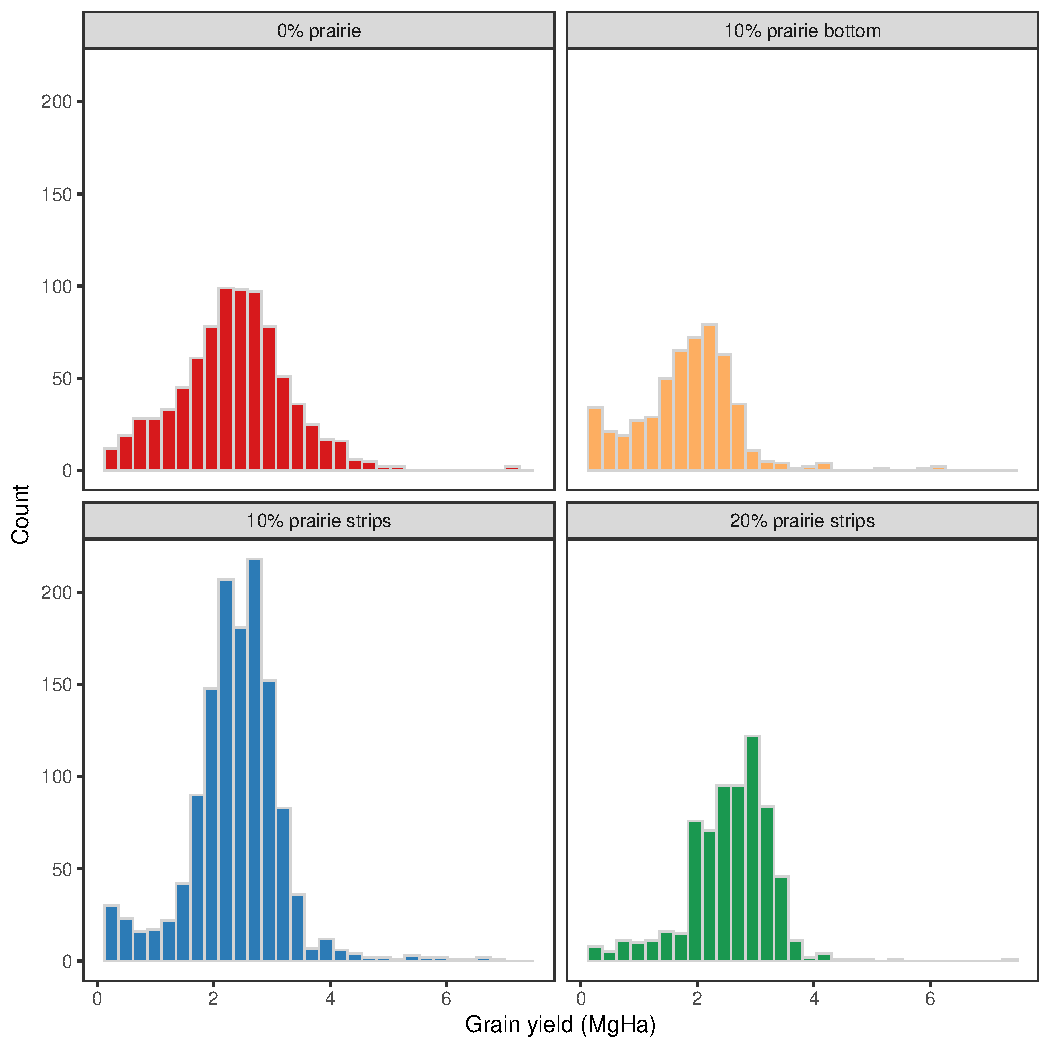
\includegraphics[width=0.55\textwidth]{./figures/strips_hist.pdf}
  \end{figure}
    
\end{frame}

\begin{frame}
  \frametitle{Context}

  \begin{center}
    What is the magnitude of crop grain yield decrease
    associated with the \textcolor{blue}{presence of prairies?}  
  \end{center}

  \begin{figure}
    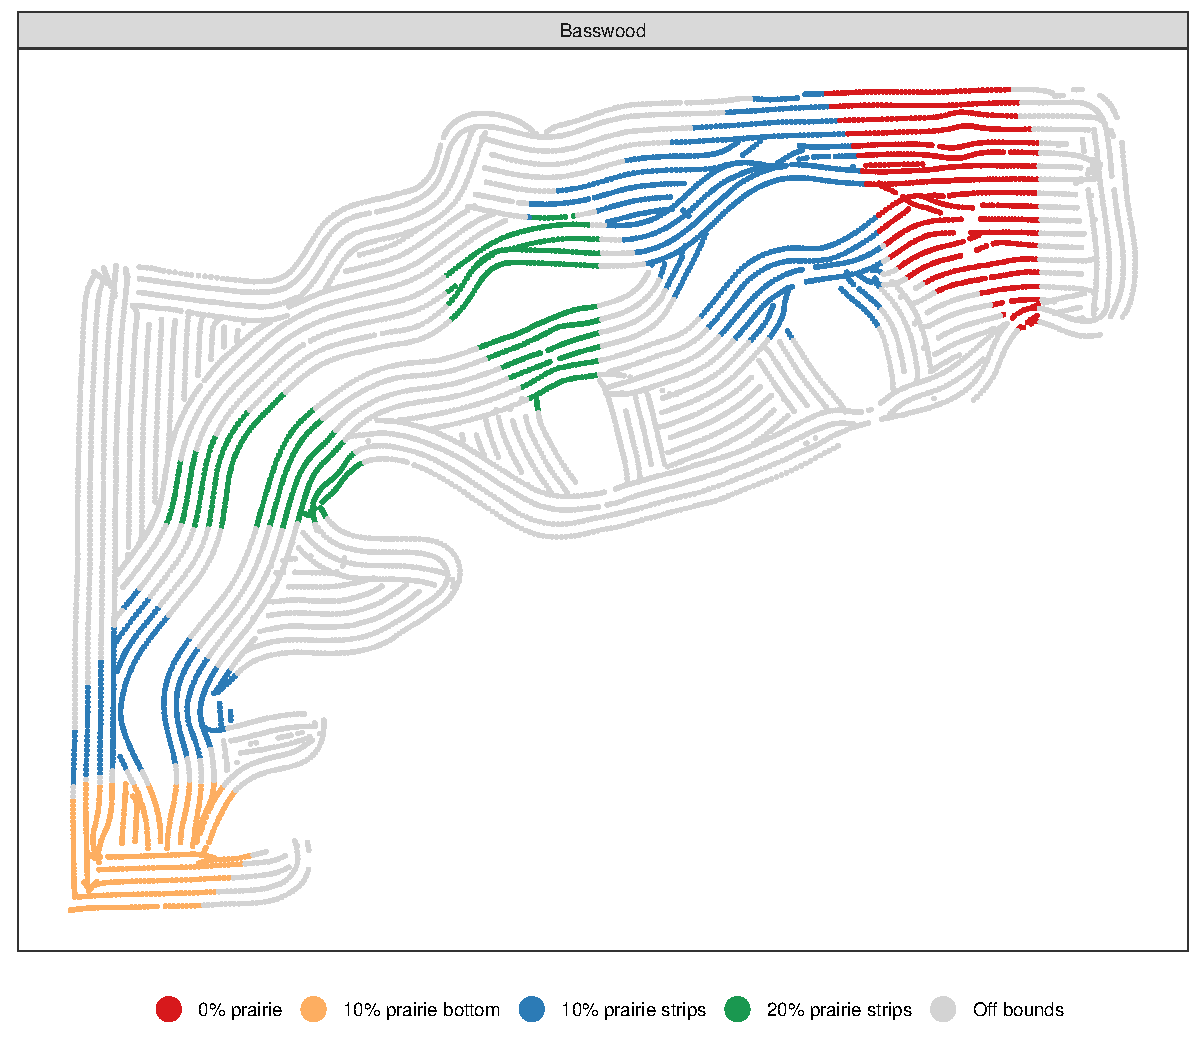
\includegraphics[width=0.65\textwidth]{./figures/strips_map.pdf}
  \end{figure}
    
\end{frame}

\begin{frame}
  \frametitle{Data acquisition}
  
  % Combine picture (internals)
  % GPS receiver picture

  \begin{figure}
    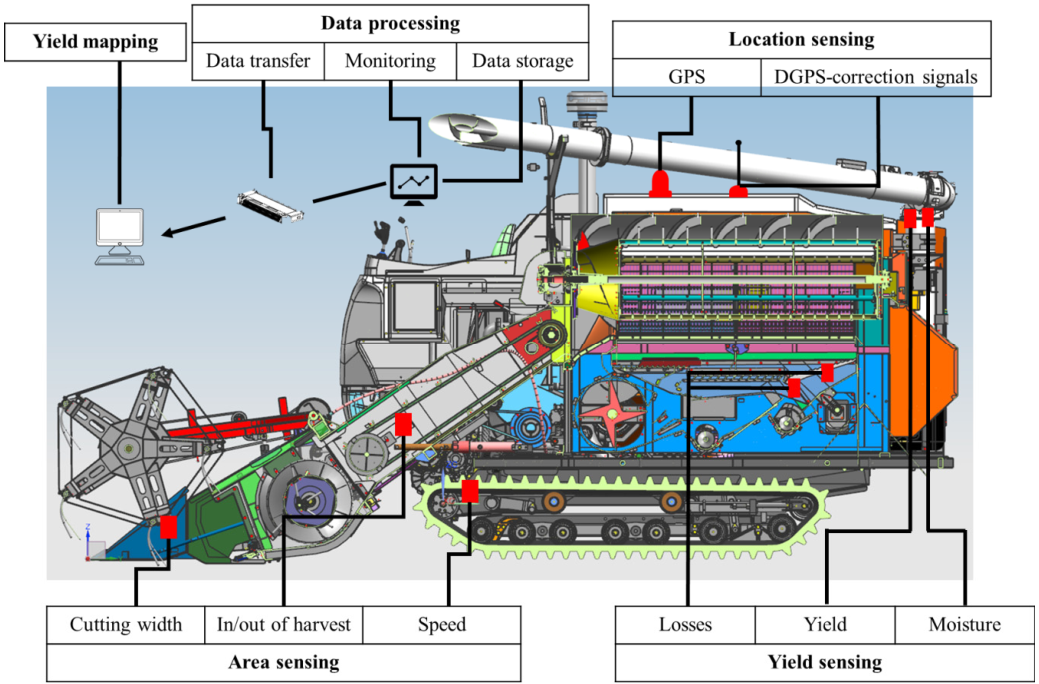
\includegraphics[width=0.95\textwidth]{./figures/combine.png}
    \caption{Yield monitoring component diagram from \ref{chungSensingTechnologiesGrain2016}}
  \end{figure}
  
\end{frame}

\begin{frame}
  \frametitle{Uncertainty map}

  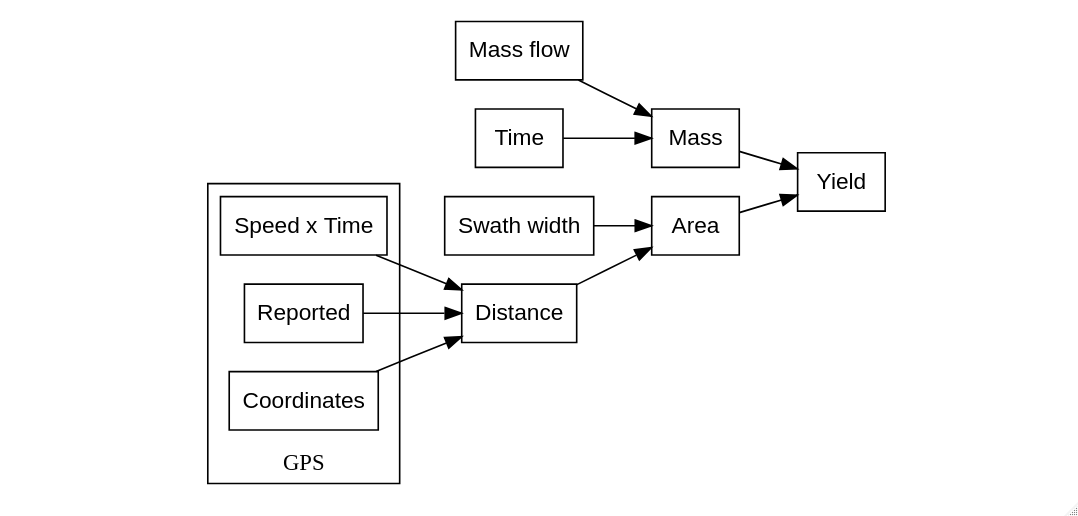
\includegraphics[width=0.95\textwidth]{./figures/uncertainty.png}
  
  % Uncertainty map
  %  Swath width (false constant), time & speed -> distance, mass,
  %  yield, time lag (different color)
  
\end{frame}

\begin{frame}
  \frametitle{Modeling challenges}

  \begin{itemize}
  \item Harvesting dynamics (time lag, start-pass and end-pass
    delay)
  \item Continuous measurements (local harvest circumstances)
  \item Positioning information (GPS receiver accuracy, repeated
    locations)
  \item Operator-induced errors (short segments, sudden speed
    changes, narrow finishes and overlaps, sharp turns, calibration)
  \end{itemize}
  
  % Show yield vs mass
  % histogram & semivariograms
  % Coefficient of variation
  % Extreme values
  % log yield vs log mass
  % Histogram of area (d * w)

\end{frame}

\begin{frame}
  \frametitle{Current analysis methodology}

  % Mention and point weaknesses  
  \begin{itemize}
  \item<2-> Normality vs non-normality
  \item<3-> Yield, but less attention to mass
  \item<4-> Yield, but less attention to log yield
  \item<5-> ``Error'' removal
    \begin{itemize}
    \item
      \onslide<6->{harvest lag time}
      \onslide<7->{, unrealistic speed}
      \onslide<8->{, short segments}
      \onslide<9->{, parallel overlaps and turns (!)}
      \onslide<10->{, biological maximum}
      \onslide<11->{, unrealistic yield}
    \end{itemize}
  \item<12-> Spatial vs non-spatial analysis
  \item<13-> Heuristics
  \end{itemize}
  
\end{frame}

%%%%%%%%%%%%%%%%%%%%%%%%%%%%%%%%%%%%%%%%%%%%%%%%%%%%%%%%%%%%%%%%%%%%%%%%%%
% The RITAS algo                                                         %
%%%%%%%%%%%%%%%%%%%%%%%%%%%%%%%%%%%%%%%%%%%%%%%%%%%%%%%%%%%%%%%%%%%%%%%%%%

\section{The RITAS algorithm}

\begin{frame}[t]
  \frametitle{RITAS}
  \framesubtitle{Notation}

  %\fontsize{6pt}{7.2}\selectfont 
  \pause
  Time-ordered observations for $t=0,\ldots,T, \ T \in \mathbb{N}$

  \pause
  \begin{itemize}
  \item<+-> mass harvested $m_t$
  \item<+-> 2-dimensional spatial coordinate $(x_t,y_t)$
  \item<+-> swath half-width $w_t$
  \item<+-> traveled distance $d_t$ (optional\footnote<+->{Not included in
      the writing, but it allows for a nice tweak next})
  \end{itemize}

\end{frame}

%%%%%%%%%%%%%%%%%%%%%%%%%%%%%%%%%%%%%%%%%%%%%%%%%%%%%%%%%%%%%%%%%%%%%%

\subsection{Rectangles}

\begin{frame}
  \frametitle{RITAS}
  \framesubtitle{Rectangles}

  \fontsize{6pt}{7.2}\selectfont 
  \begin{columns}[T]
    \begin{column}{0.30\textwidth}
      \only<2->{
        Consider two subsequent locations $\mathbf{s_t}, \mathbf{s_{t-1}}$
      }

      \vspace{5px}
      
      \only<3->{
        Compute the linear displacement vector slope:
        \begin{align*}
          b_t &= \frac{(y_t - y_{t-1})}{(x_t - x_{t-1})}
        \end{align*}
      }

      \vspace{5px}
      
      \only<4->{
        Define
        \begin{align*}
          dx_t &= w_t (1 + b_t^{-2})^{-\frac{1}{2}} \\
          dy_t &= - dx_t b_t^{-1}
        \end{align*}
      }

      \vspace{5px}
      
      \only<5->{
        Compute the vertices $\{(x_{i} \pm dx_t, y_{i} \pm dy_t):
        i = t, t-1\}$
      }

      \vspace{10px}
      
      \only<6->{
        \begin{alertblock}{Rectangle collection}
          $\mathcal{P} = \{P_{\tau}$: $\tau \in \{1, \dots, T\}\}$
        \end{alertblock}
      }
    \end{column}
    
    \begin{column}{0.70\textwidth}
      \begin{center}
        \only<2>{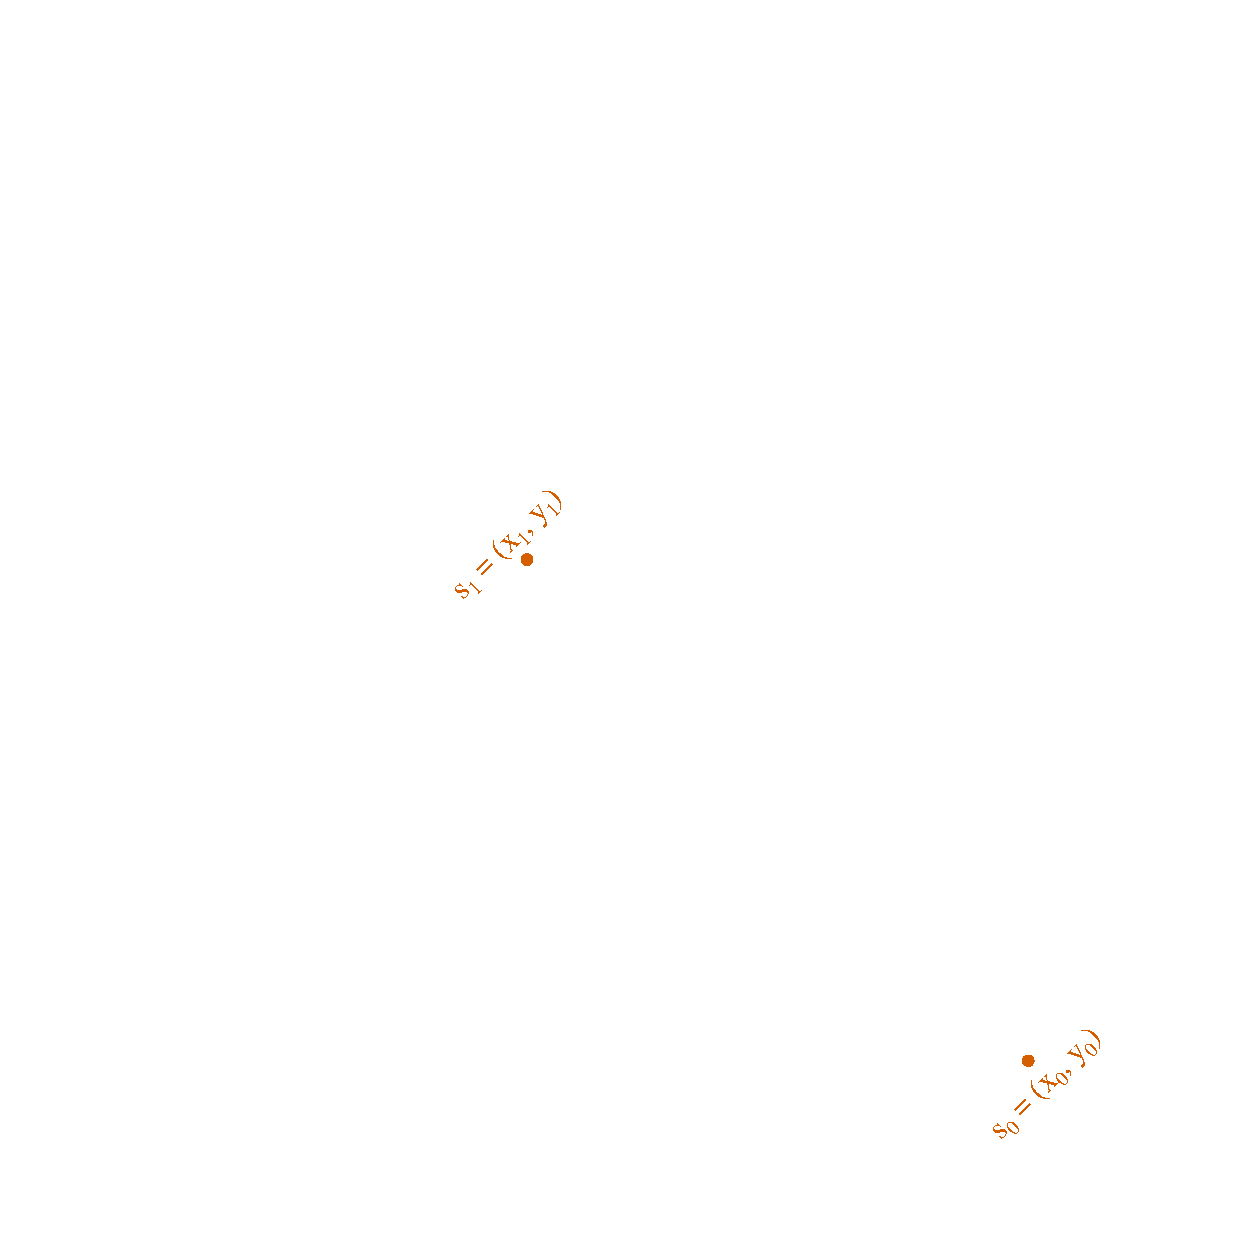
\includegraphics[width=0.95\textwidth]{./figures/intro_rectangles_1}}
        \only<3>{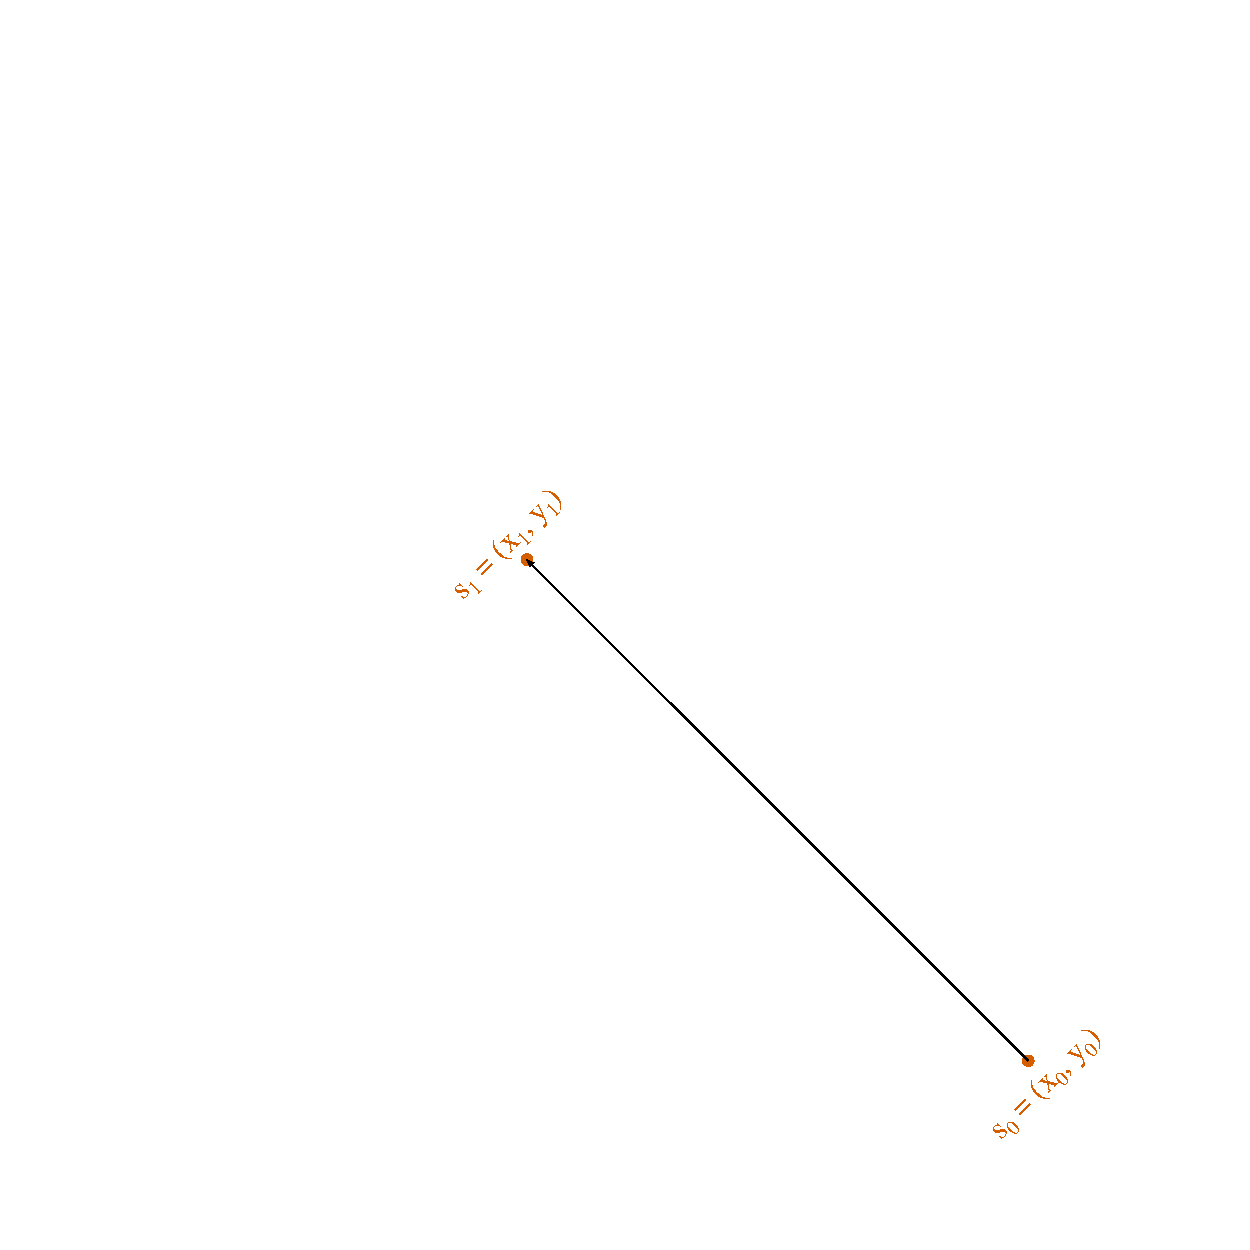
\includegraphics[width=0.95\textwidth]{./figures/intro_rectangles_2}}
        \only<4>{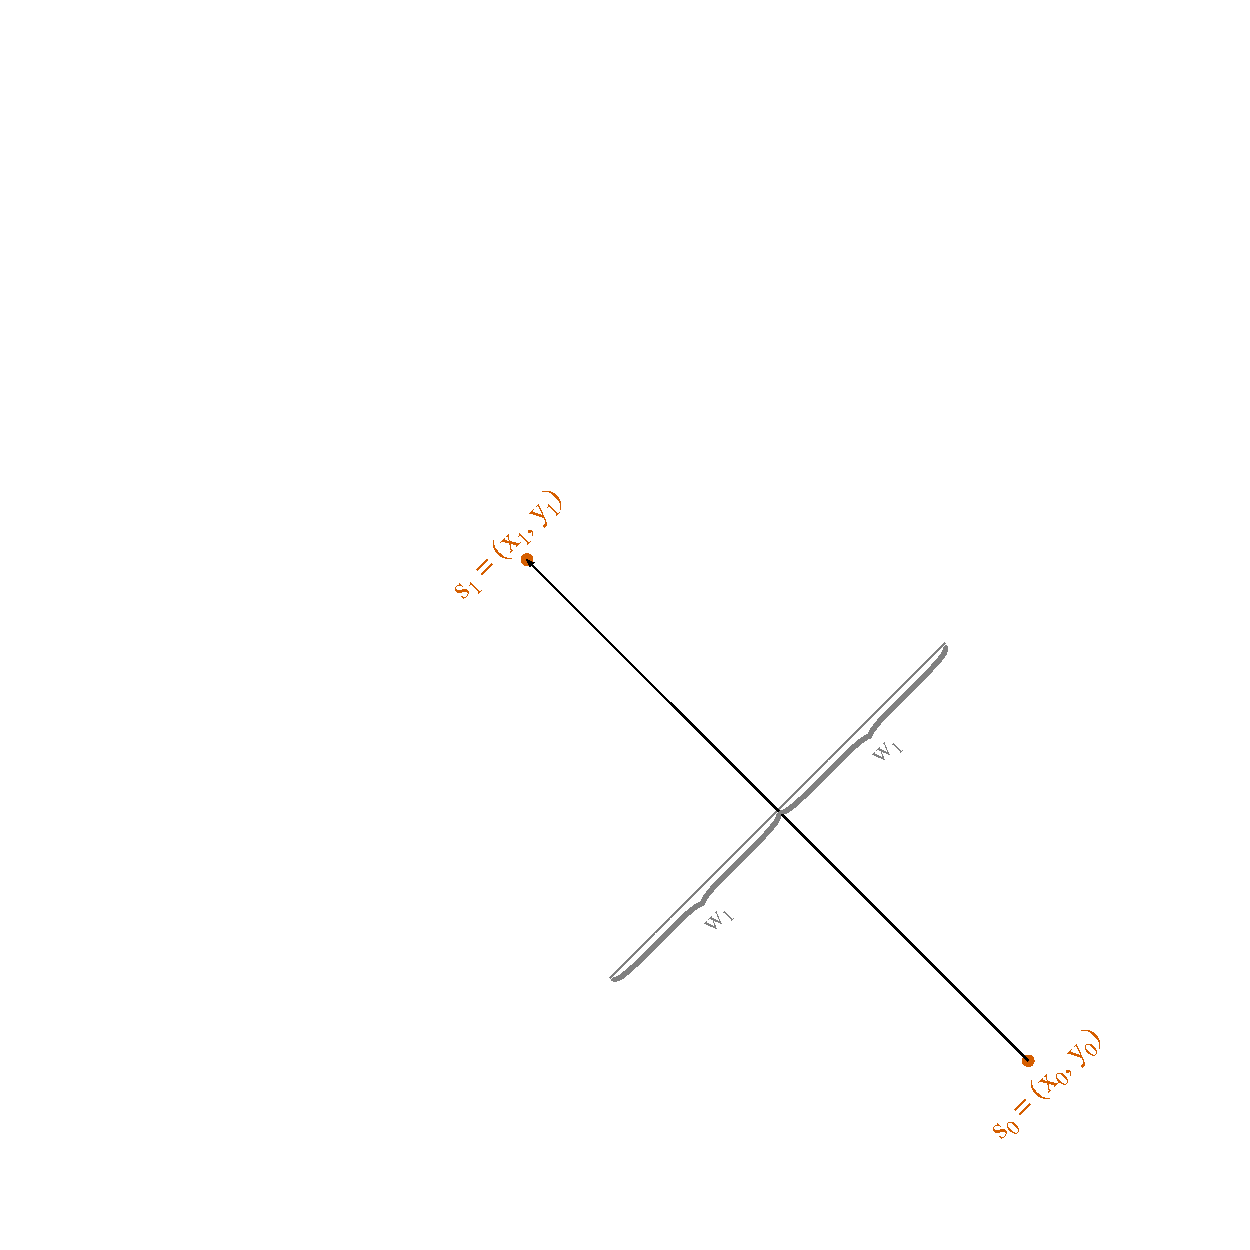
\includegraphics[width=0.95\textwidth]{./figures/intro_rectangles_3}}
        \only<5>{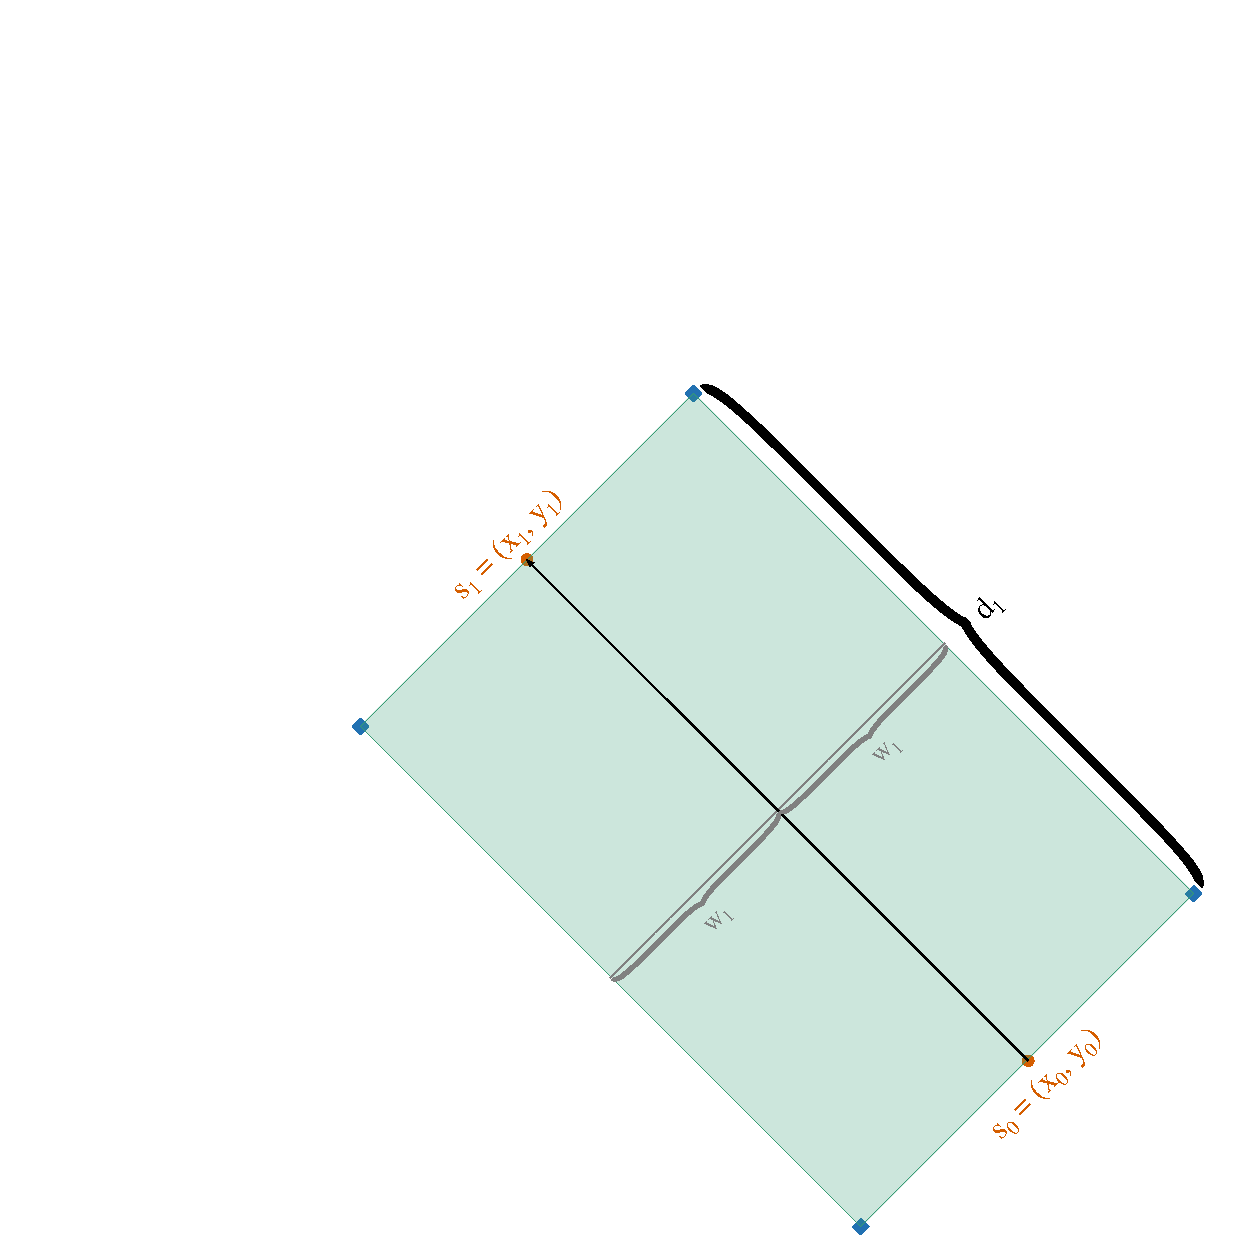
\includegraphics[width=0.95\textwidth]{./figures/intro_rectangles_4}}
        \only<6>{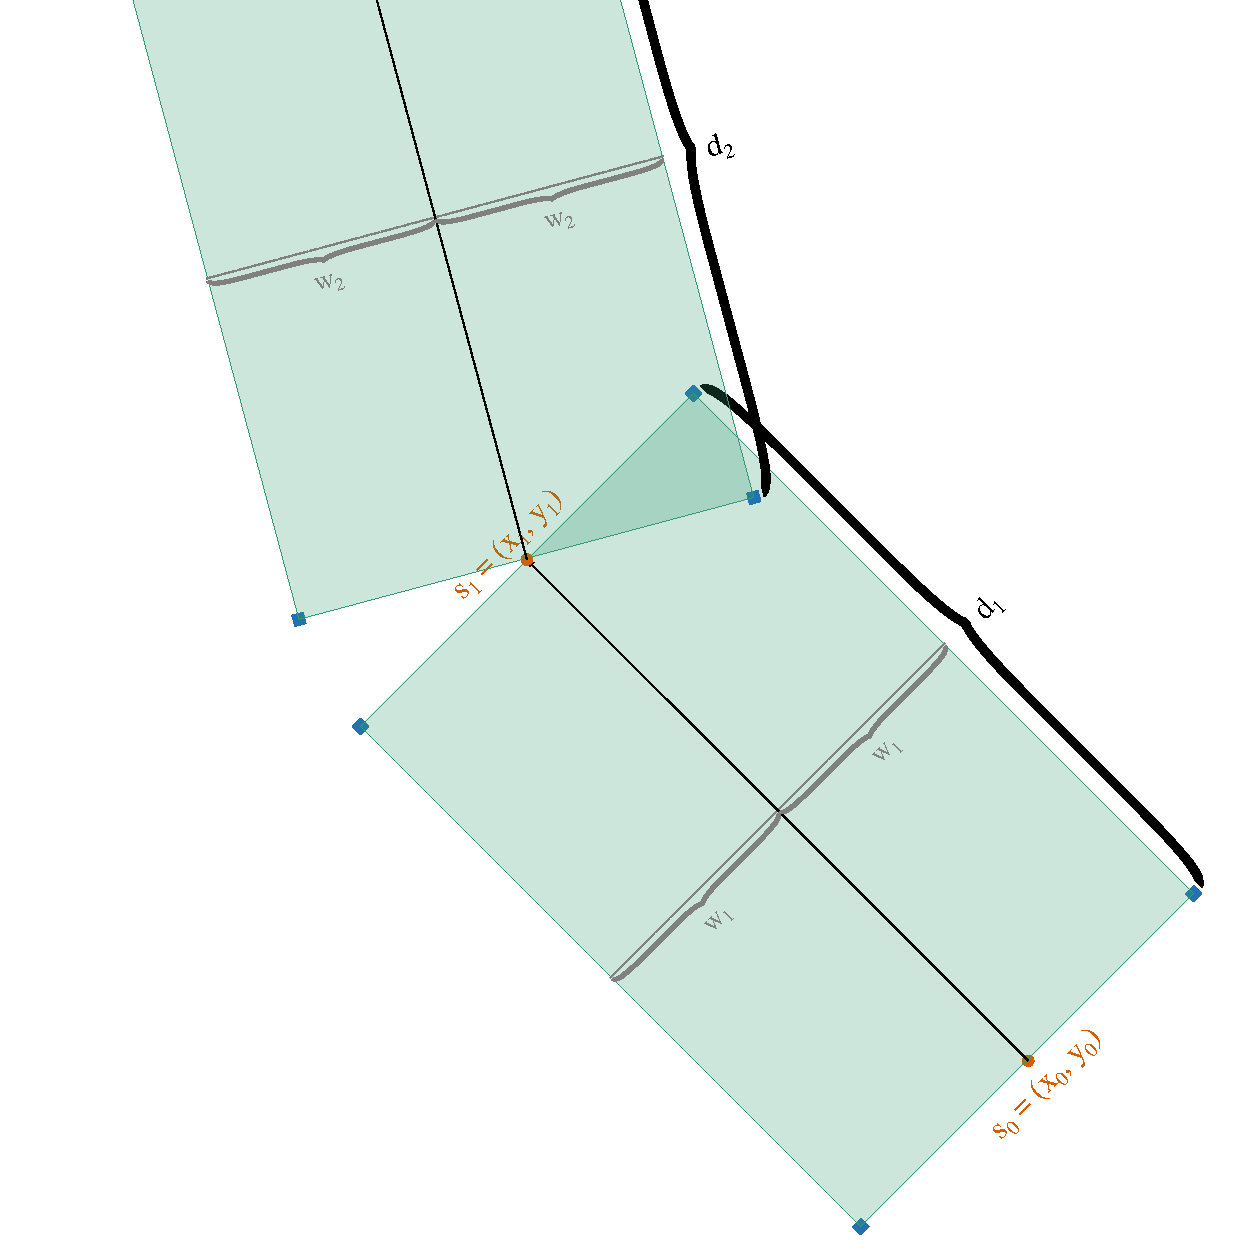
\includegraphics[width=0.95\textwidth]{./figures/intro_rectangles}}
      \end{center}
    \end{column}
  \end{columns}
\end{frame}

%%%%%%%%%%%%%%%%%%%%%%%%%%%%%%%%%%%%%%%%%%%%%%%%%%%%%%%%%%%%%%%%%%%%%%

\subsection{Intersection}

\begin{frame}
  \frametitle{RITAS}
  \framesubtitle{Intersection}

  \fontsize{6pt}{7.2}\selectfont 
  \begin{columns}[T]
    \begin{column}{0.30\textwidth}

    \end{column}
    
    \begin{column}{0.70\textwidth}
      \begin{center}
        \includegraphics<1->[width=0.95\textwidth]{./figures/intro_intersection}
      \end{center}
    \end{column}
  \end{columns}
\end{frame}

%%%%%%%%%%%%%%%%%%%%%%%%%%%%%%%%%%%%%%%%%%%%%%%%%%%%%%%%%%%%%%%%%%%%%%

\subsection{Tessellation}

\begin{frame}
  \frametitle{RITAS}
  \framesubtitle{Tessellation}

  \fontsize{6pt}{7.2}\selectfont 
  \begin{columns}[T]
    \begin{column}{0.30\textwidth}

      \onslide<2->{
        Define the time-ordered relative complement
        
        \begin{align*}
          \tilde{P}_\tau = P_t \setminus \left( \bigcup_{i = 1}^{t - 1} P_i
          \right)
        \end{align*}
      }
    
      \vspace{105px}
      \begin{alertblock}{Tessellation collection}<3->
        $\mathcal{\tilde{P}} = \{\tilde{P}_{\tau}$: $\tau \in \{1, \dots, T\}\}$
      \end{alertblock}
      
    \end{column}
    
    \begin{column}{0.70\textwidth}
      \begin{center}
        \includegraphics<1->[width=0.95\textwidth]{./figures/intro_tessellation}
      \end{center}
    \end{column}
  \end{columns}
\end{frame}

%%%%%%%%%%%%%%%%%%%%%%%%%%%%%%%%%%%%%%%%%%%%%%%%%%%%%%%%%%%%%%%%%%%%%%

\subsection{Aggregation}

\begin{frame}
  \frametitle{RITAS}
  \framesubtitle{Apportioning}

  \fontsize{6pt}{7.2}\selectfont 
  \begin{columns}[T]
    \begin{column}{0.30\textwidth}
      \only<2->{
        Fix $N \in \mathbb{N}$
      }

      \vspace{5px}
      
      \only<3->{
        Create $N$ equally-sized, non-overlapping, contiguous
        squares covering $\mathcal{\tilde{P}}$
      }

      \vspace{5px}
      
      \only<4->{
        Compute the pairwise overlapping area proportion $\pi_{\tau,
          n} \in [0, 1]$ between $\tau$-th non-overlapping polygon
        $\tilde{P}_{\tau}$ and the n$-th$ pixel for $\tau \in \{1,
        \dots, T\}$ and $n \in \{1, \dots, N\}$        
      }

      \vspace{5px}

      \only<5->{
        Assign $m^{*}_n = \sum_{\tau = 1}^{T} \pi_{\tau, n} m_{\tau}$ to
        the $n$-th pixel
      }

      \vspace{5px}
      
      \only<6->{
        Upweight $m^{*}_n$ by $\sum_{\tau = 1}^{T} \pi_{\tau, n}$ (optional)
      }

      \vspace{50px}
      
      \only<7->{
        \begin{alertblock}{Grid collection}
          $\mathcal{P^*} = \{P^*_{\tau}$: $\tau \in \{1, \dots, T\}\}$
        \end{alertblock}
      }
  \end{column}
    
    \begin{column}{0.70\textwidth}
      \begin{center}
        \includegraphics<1->[width=0.95\textwidth]{./figures/intro_apportioning}
      \end{center}
    \end{column}
  \end{columns}
\end{frame}

%%%%%%%%%%%%%%%%%%%%%%%%%%%%%%%%%%%%%%%%%%%%%%%%%%%%%%%%%%%%%%%%%%%%%%

\subsection{Smoothing}

\begin{frame}
  \frametitle{RITAS}
  \framesubtitle{Smoothing}

  \fontsize{6pt}{7.2}\selectfont 
  \begin{columns}[T]
    \begin{column}{0.30\textwidth}
      \begin{itemize}
      \item<2-> Model
      \item<3-> Inference
      \item<4-> Prediction
      \end{itemize}
    \end{column}
    
    \begin{column}{0.70\textwidth}
      \begin{center}
        \includegraphics<1->[width=0.95\textwidth]{./figures/intro_smoothing}
      \end{center}
    \end{column}
  \end{columns}

\end{frame}

\begin{frame}[t]

  \frametitle{RITAS}
  \framesubtitle{Smoothing}

  \onslide<2-4>{
    \alert{Model}
    \begin{equation*}
      f(\mathbf{S}) \triangleq \log(\mathbf{m}) \sim \mathcal{G}
      \mathcal{P}\left(m(\mathbf{S}), k\left(\mathbf{S},
          \mathbf{S}^{\prime}\right)\right)
    \end{equation*}
  }
  \onslide<3-4>{
    \begin{equation*}
      k(d)=\frac{2^{1-\nu}}{\Gamma(\nu)}\left(\frac{\sqrt{2
            \nu}d}{\ell}\right)^{\nu} K_{\nu}\left(\frac{\sqrt{2
            \nu}d}{\ell}\right)
    \end{equation*}
    for $d \ge 0$ known and fixed, $\ell, \nu > 0$ unknown
  }

  \onslide<4>{
    \alert{Log marginal likelihood}
    \begin{equation*}
      \log p(\mathbf{m} \mid \mathbf{S})=-\frac{1}{2}
      \mathbf{y}^{\top}\left(K+\sigma_{n}^{2} I\right)^{-1}
      \mathbf{y}-\frac{1}{2} \log \left|K+\sigma_{n}^{2}
        I\right|-\frac{n}{2} \log 2 \pi    
    \end{equation*}
    for $K = k\left(\mathbf{S}, \mathbf{S}^{\prime}\right)$
  }
  
\end{frame}

\begin{frame}[t]
  \frametitle{RITAS}
  \framesubtitle{Smoothing}
  
  \onslide<1->{
    \alert{Predictive distribution}
    \begin{equation*}
      \left[
        \begin{array}{c}
          \mathbf{m} \\
          \mathbf{f}_{*}
        \end{array}
      \right]
      \sim
      \mathcal{N}
      \left(
        \mathbf{0},
        \left[
          \begin{array}{cc}
            K(S, S)+\sigma_{n}^{2} I & K\left(S, S_{*}\right) \\
            K\left(S_{*}, S\right)& K\left(S_{*}, S_{*}\right)
          \end{array}
        \right]
      \right)
    \end{equation*}
  }

  \onslide<2->{
    \begin{equation*}
      \begin{aligned}
        \mathbf{f}_{*} \mid S, \mathbf{m}, S_{*} & \sim
        \mathcal{N}\left(\mu_{\ell}, \sigma^2_{\ell}\right), \text {
          where } \\
        \mu_{f} &=
        K\left(S_{*}, S\right)\left[K(S,
          S)+\sigma_{n}^{2} I\right]^{-1} \mathbf{y} \\
        \sigma^2_{f}  &=K\left(S_{*},
          S_{*}\right)-K\left(S_{*}, S\right)\left[K(S,
          S)+\sigma_{n}^{2} I\right]^{-1} K\left(S, S_{*}\right)
      \end{aligned}
    \end{equation*}
  }
  
  \onslide<3->{
    \begin{equation*}
      \mu_{m} = \exp\left(\mu_{f} +
        {\sigma}^2_{f}/2\right) \quad\mbox{and}\quad
      {\sigma}^2_{m} = \exp\left(2 {\mu}_{f} +
        {\sigma}^2_{f}\right)
      \left[\exp\left({\sigma}^2_{f}\right) - 1\right]
    \end{equation*}
  }

\end{frame}

\begin{frame}
  \frametitle{Implementation}

  % R package, discuss kappa, computing time, etc
  
  \begin{itemize}
  \item<2-> R package, documentation at about 80\%
  \item<3-> Smoothing
    \begin{itemize}
    \item<4-> Prediction parallelization via \textit{doParallel} and
      \textit{foreach}
    \item<5-> Can limit the number of neighboring points to speed up prediction 
    \end{itemize}
  \item<6-> Polygon operations using \textit{rgeos}, an R interface to
    \textit{Geometry Engine, Open Source} written in C++
  \item<7-> Smoothing using the \textit{gstat} package
    \begin{itemize}
    \item<8-> Not maintained anymore, should be replaced
    \item<9-> Has issues with small $\nu < 0.3$
    \end{itemize}
  \end{itemize}

\end{frame}

\begin{frame}[fragile]
  \frametitle{Code snippet}

  \scriptsize
  \begin{verbatim}
proj4string <-
  "+proj=utm +zone=15 +datum=WGS84 +units=m +ellps=WGS84 +towgs84=0,0,0"

> head(DF)
      site year record        x       y  mass swath    d
1 Basswood 2012      0 476877.0 4598424  3.67  6.09   NA
2 Basswood 2012      1 476879.5 4598424  7.87  6.09 1.87
3 Basswood 2012      2 476881.8 4598424  2.65  6.09 2.33
4 Basswood 2012      3 476882.6 4598424  9.26  6.09 0.76
5 Basswood 2012      4 476884.8 4598424 11.68  6.09 2.26
6 Basswood 2012      5 476887.0 4598424 18.14  6.09 2.23

ritas(DF, proj4string, "Basswood", 2012, res = 5, nmax = 0.4, nCores = 16)
\end{verbatim}

\end{frame}

%%%%%%%%%%%%%%%%%%%%%%%%%%%%%%%%%%%%%%%%%%%%%%%%%%%%%%%%%%%%%%%%%%%%%%%%%%
% STRIPS                                                                 %
%%%%%%%%%%%%%%%%%%%%%%%%%%%%%%%%%%%%%%%%%%%%%%%%%%%%%%%%%%%%%%%%%%%%%%%%%%

\section{STRIPS}

\begin{frame}
  \frametitle{Data set}

  \begin{center}
    \only<1>{\includegraphics[width=0.95\textwidth]{./figures/data}}
  \end{center}

  % Description of the dataset
  
\end{frame}

\begin{frame}
  \frametitle{Results}

  % Maps -- maybe step by step
  % Gif

  \begin{center}
    \only<1>{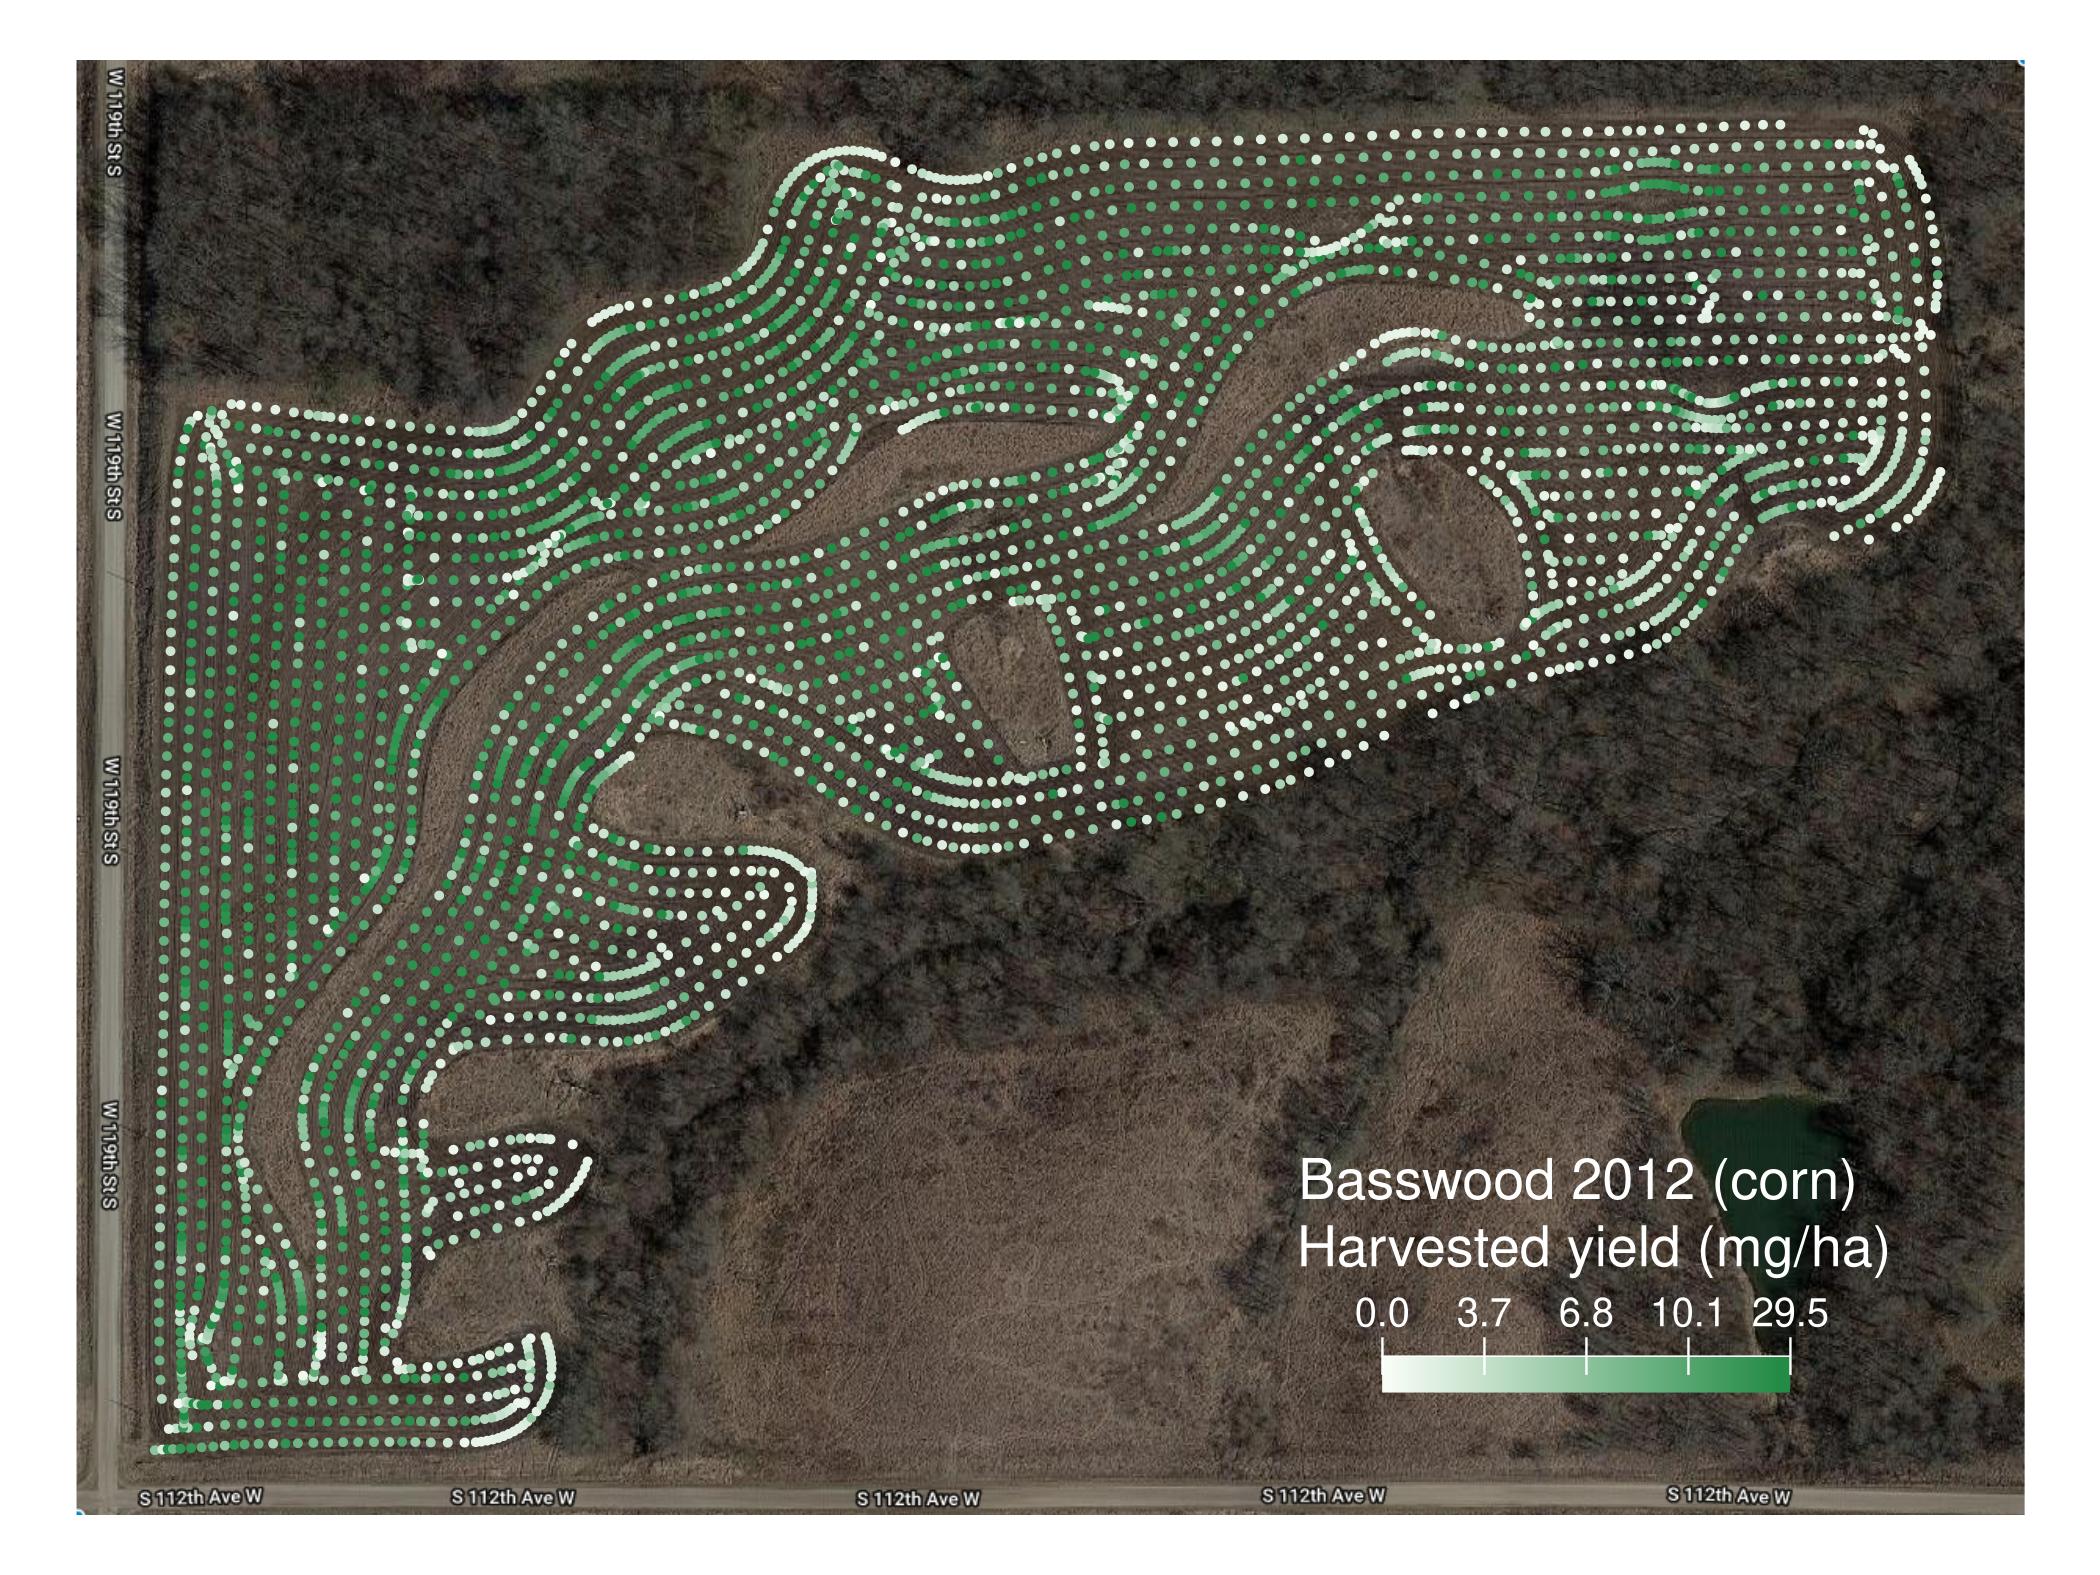
\includegraphics[width=0.95\textwidth]{./figures/maps/basswood_2012_01_points.png}}
    \only<2>{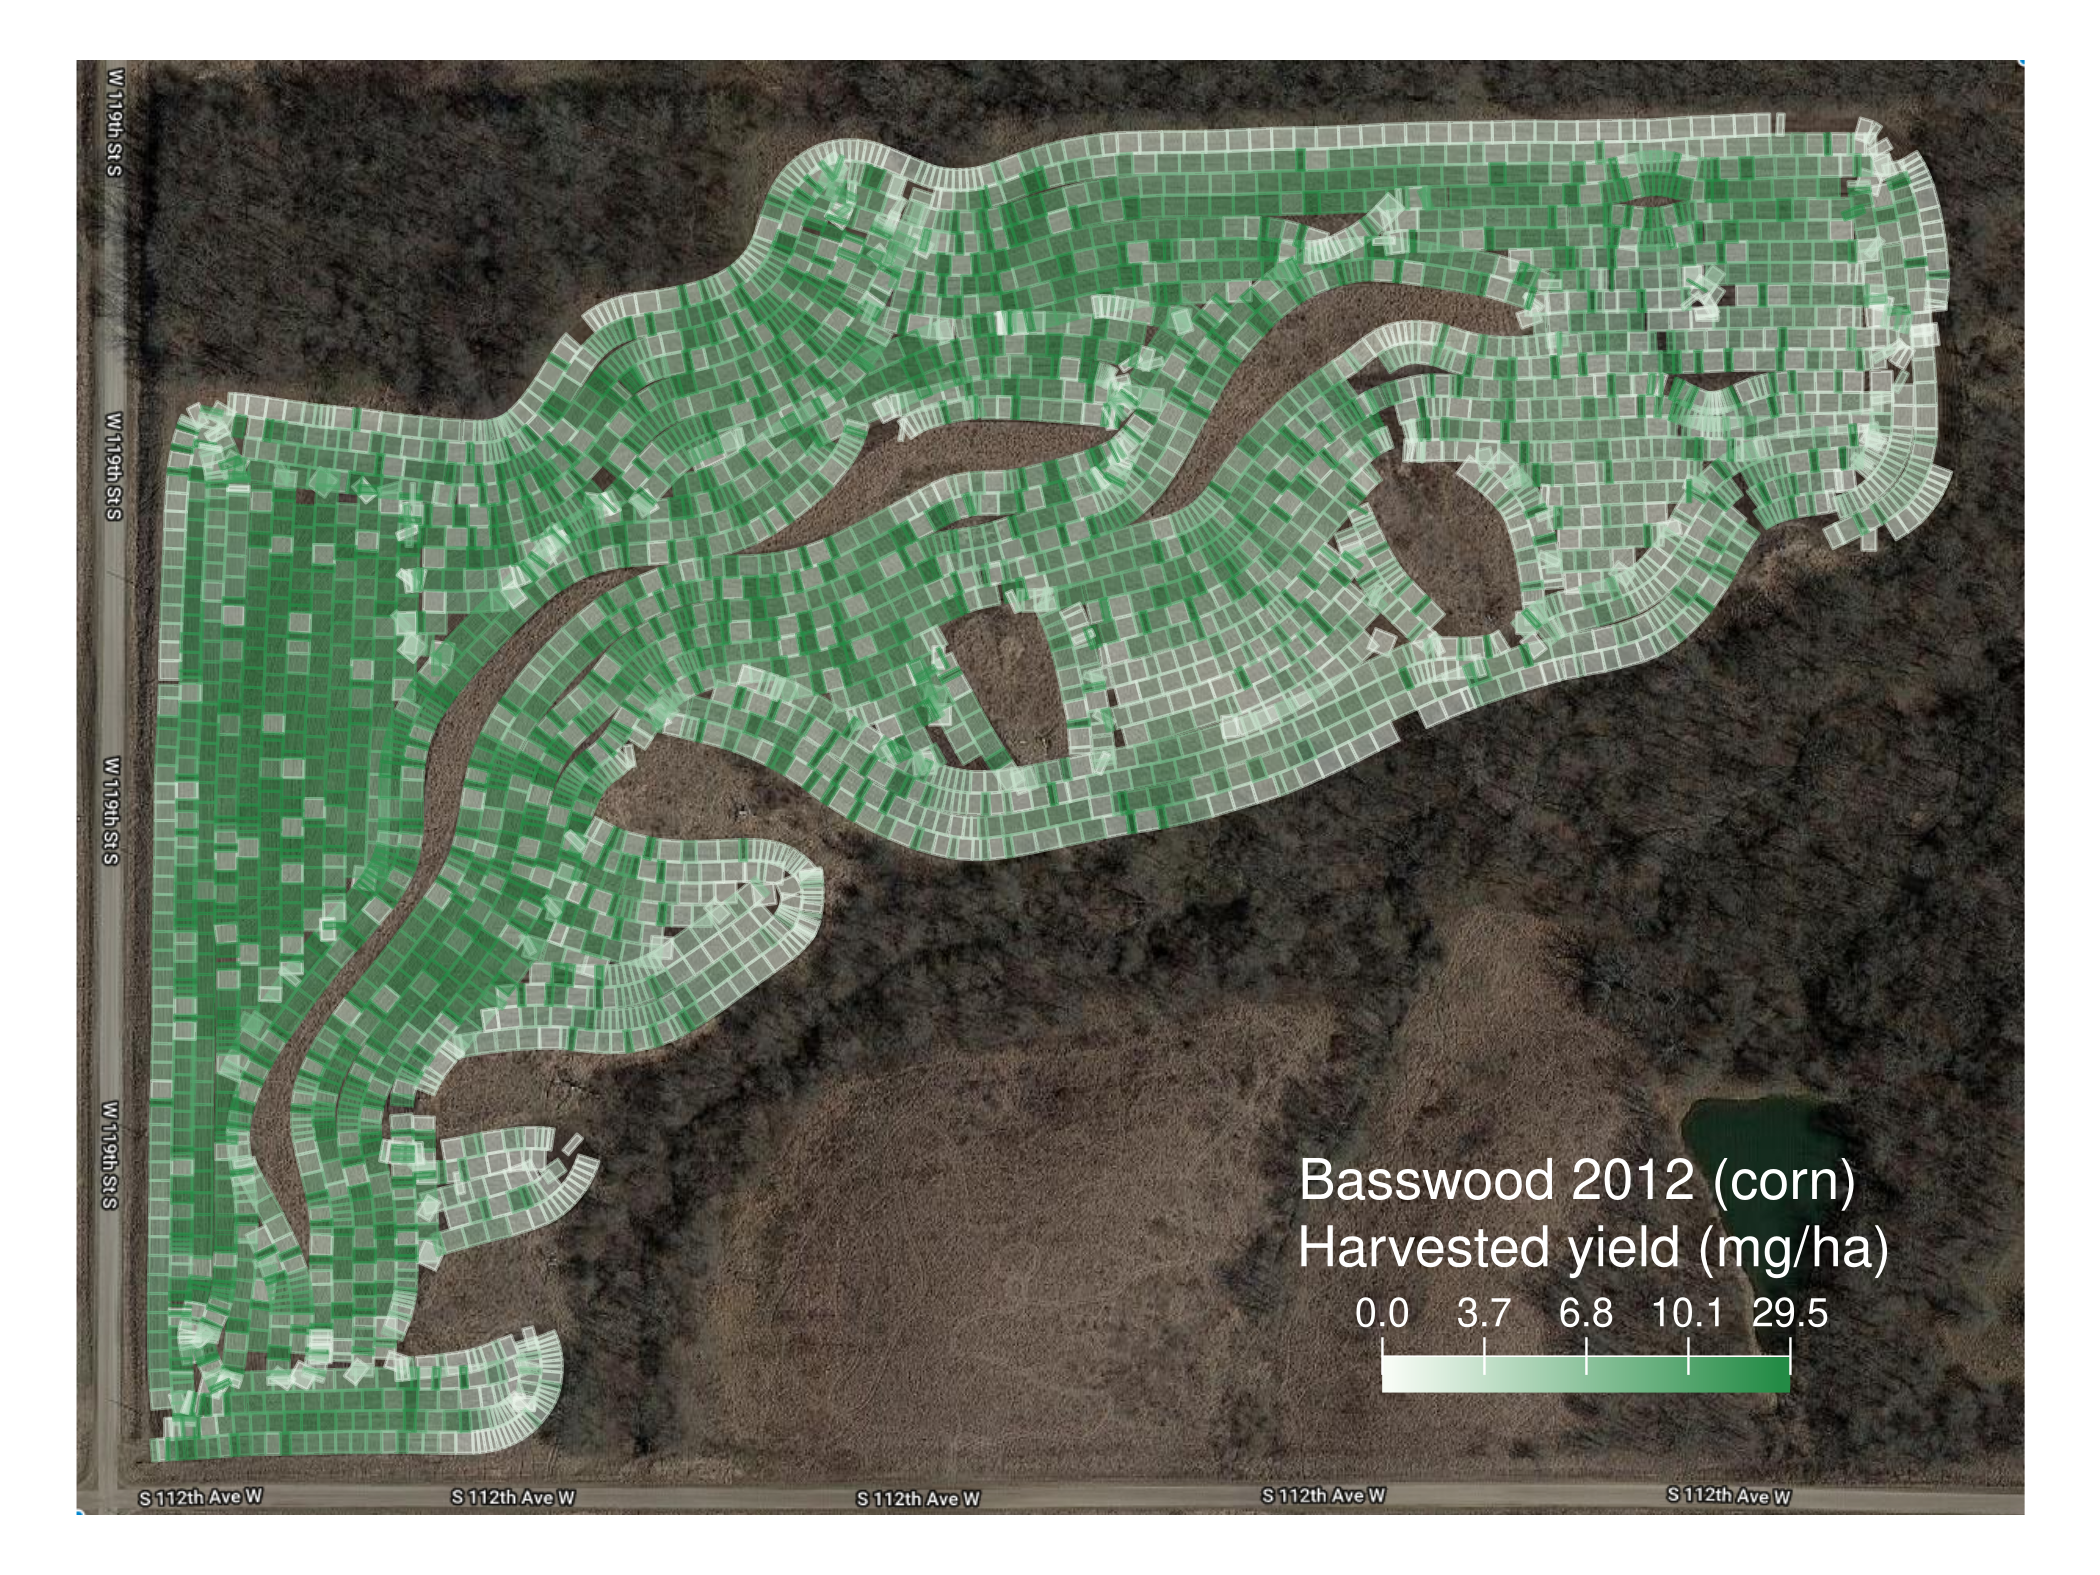
\includegraphics[width=0.95\textwidth]{./figures/maps/basswood_2012_02_rectangles.png}}
    \only<3>{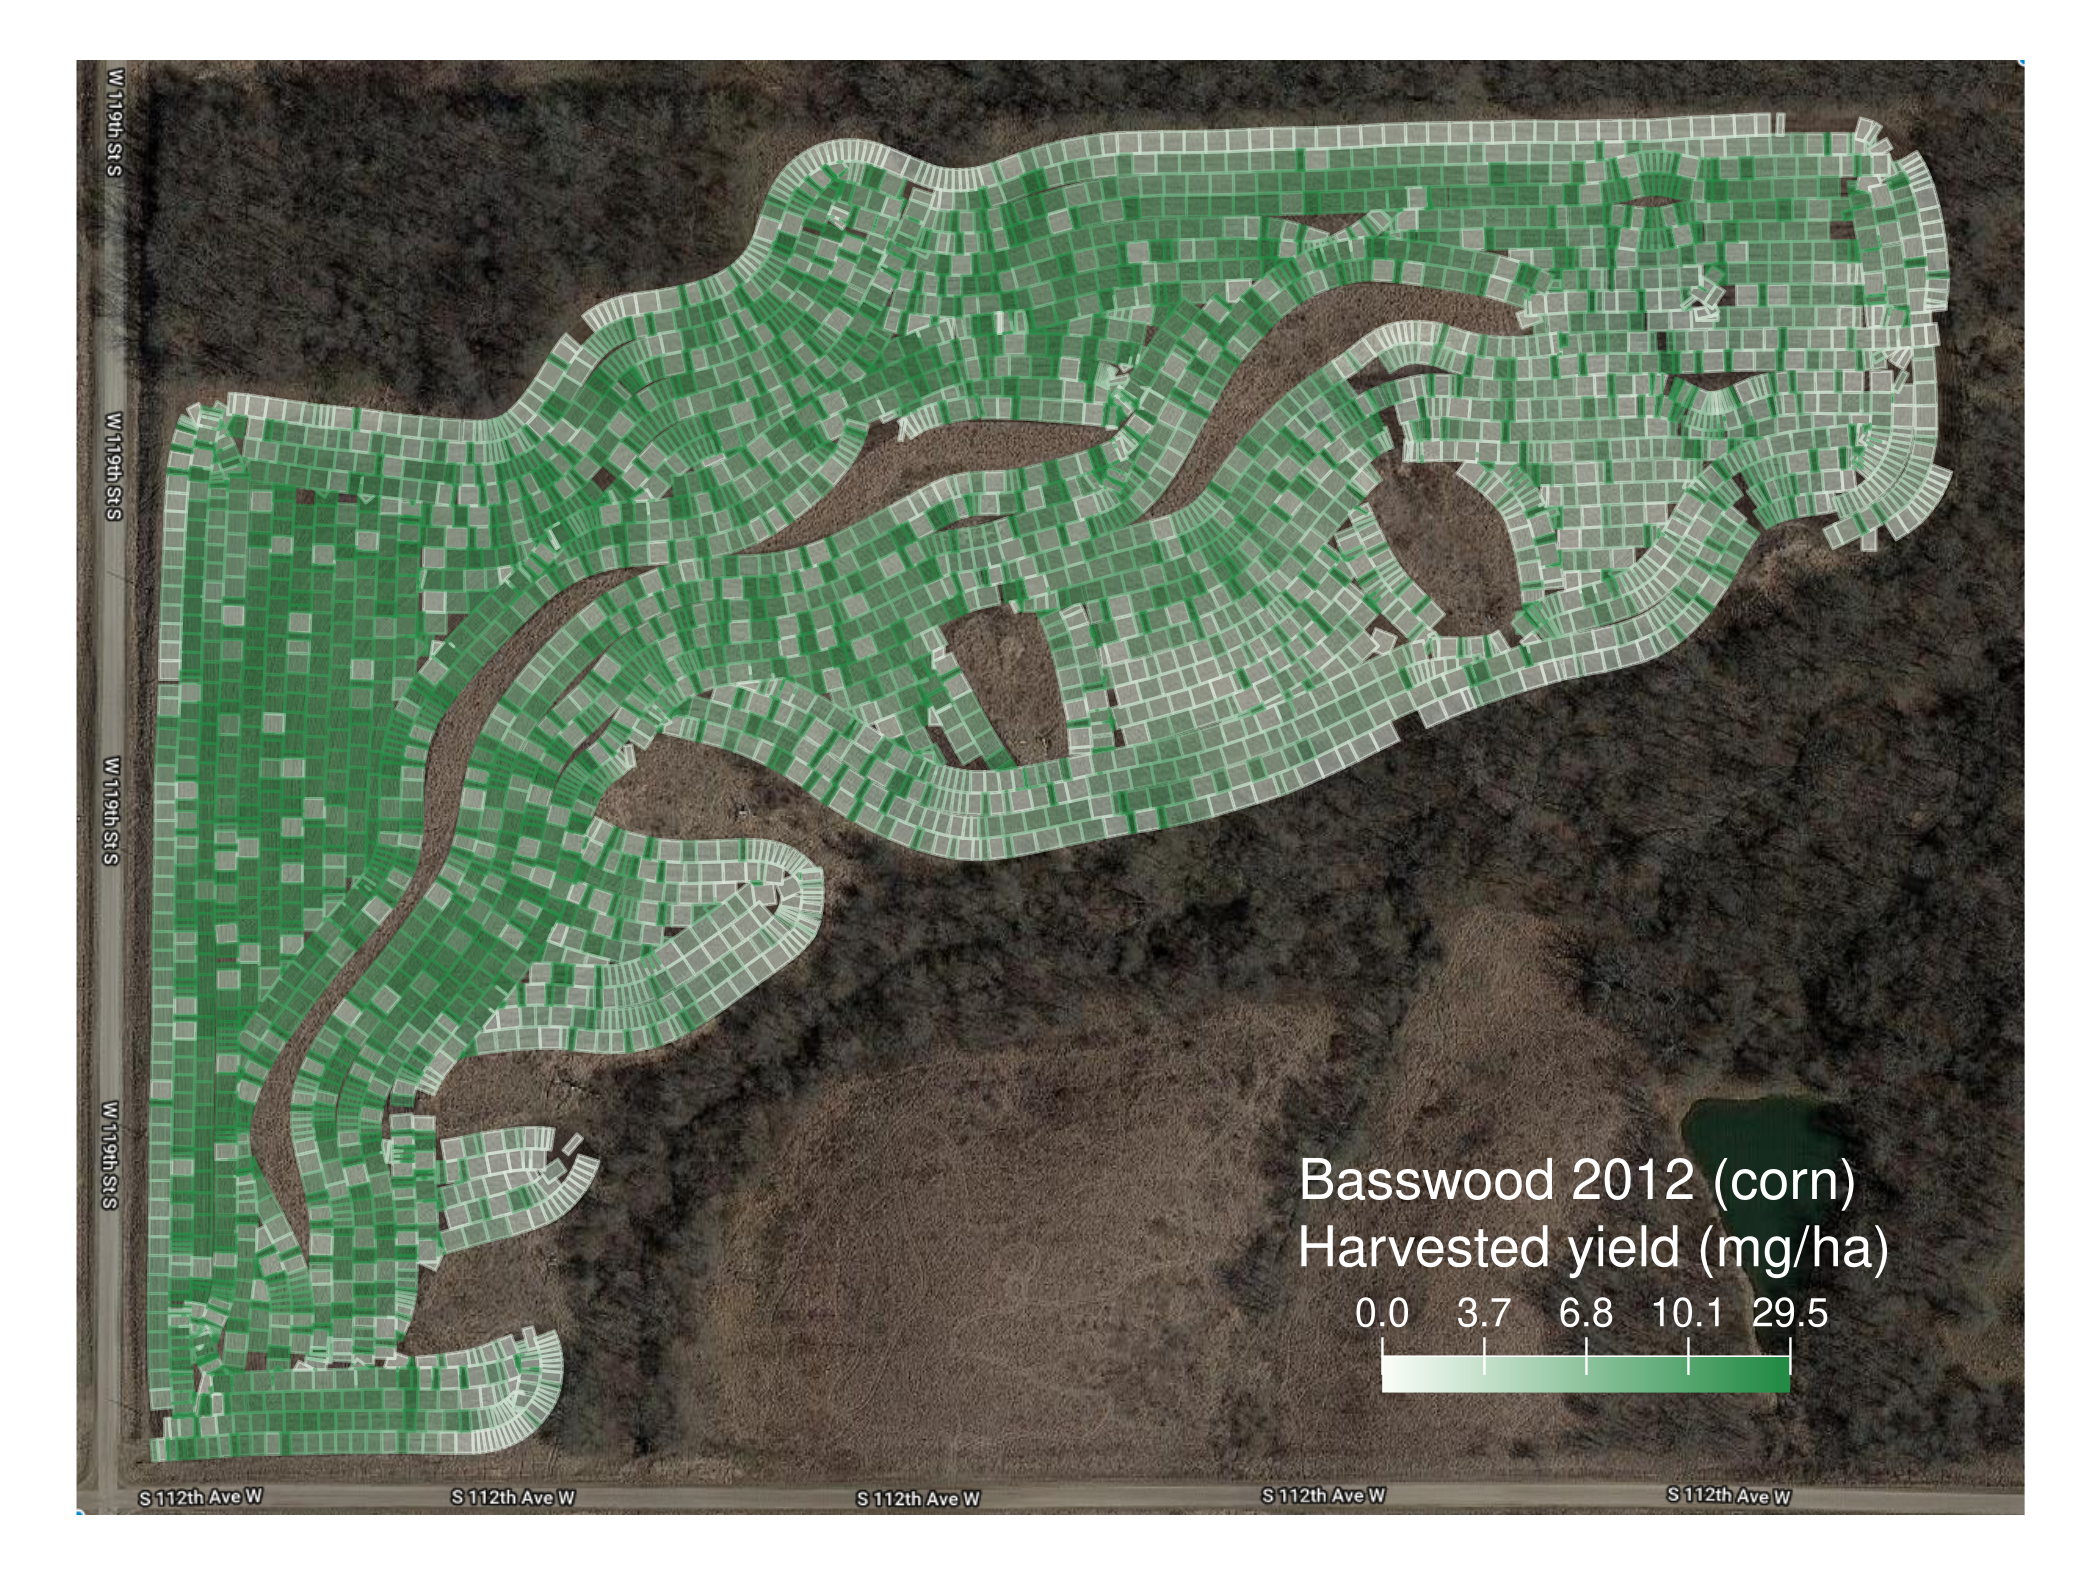
\includegraphics[width=0.95\textwidth]{./figures/maps/basswood_2012_03_tessellation.png}}
    \only<4>{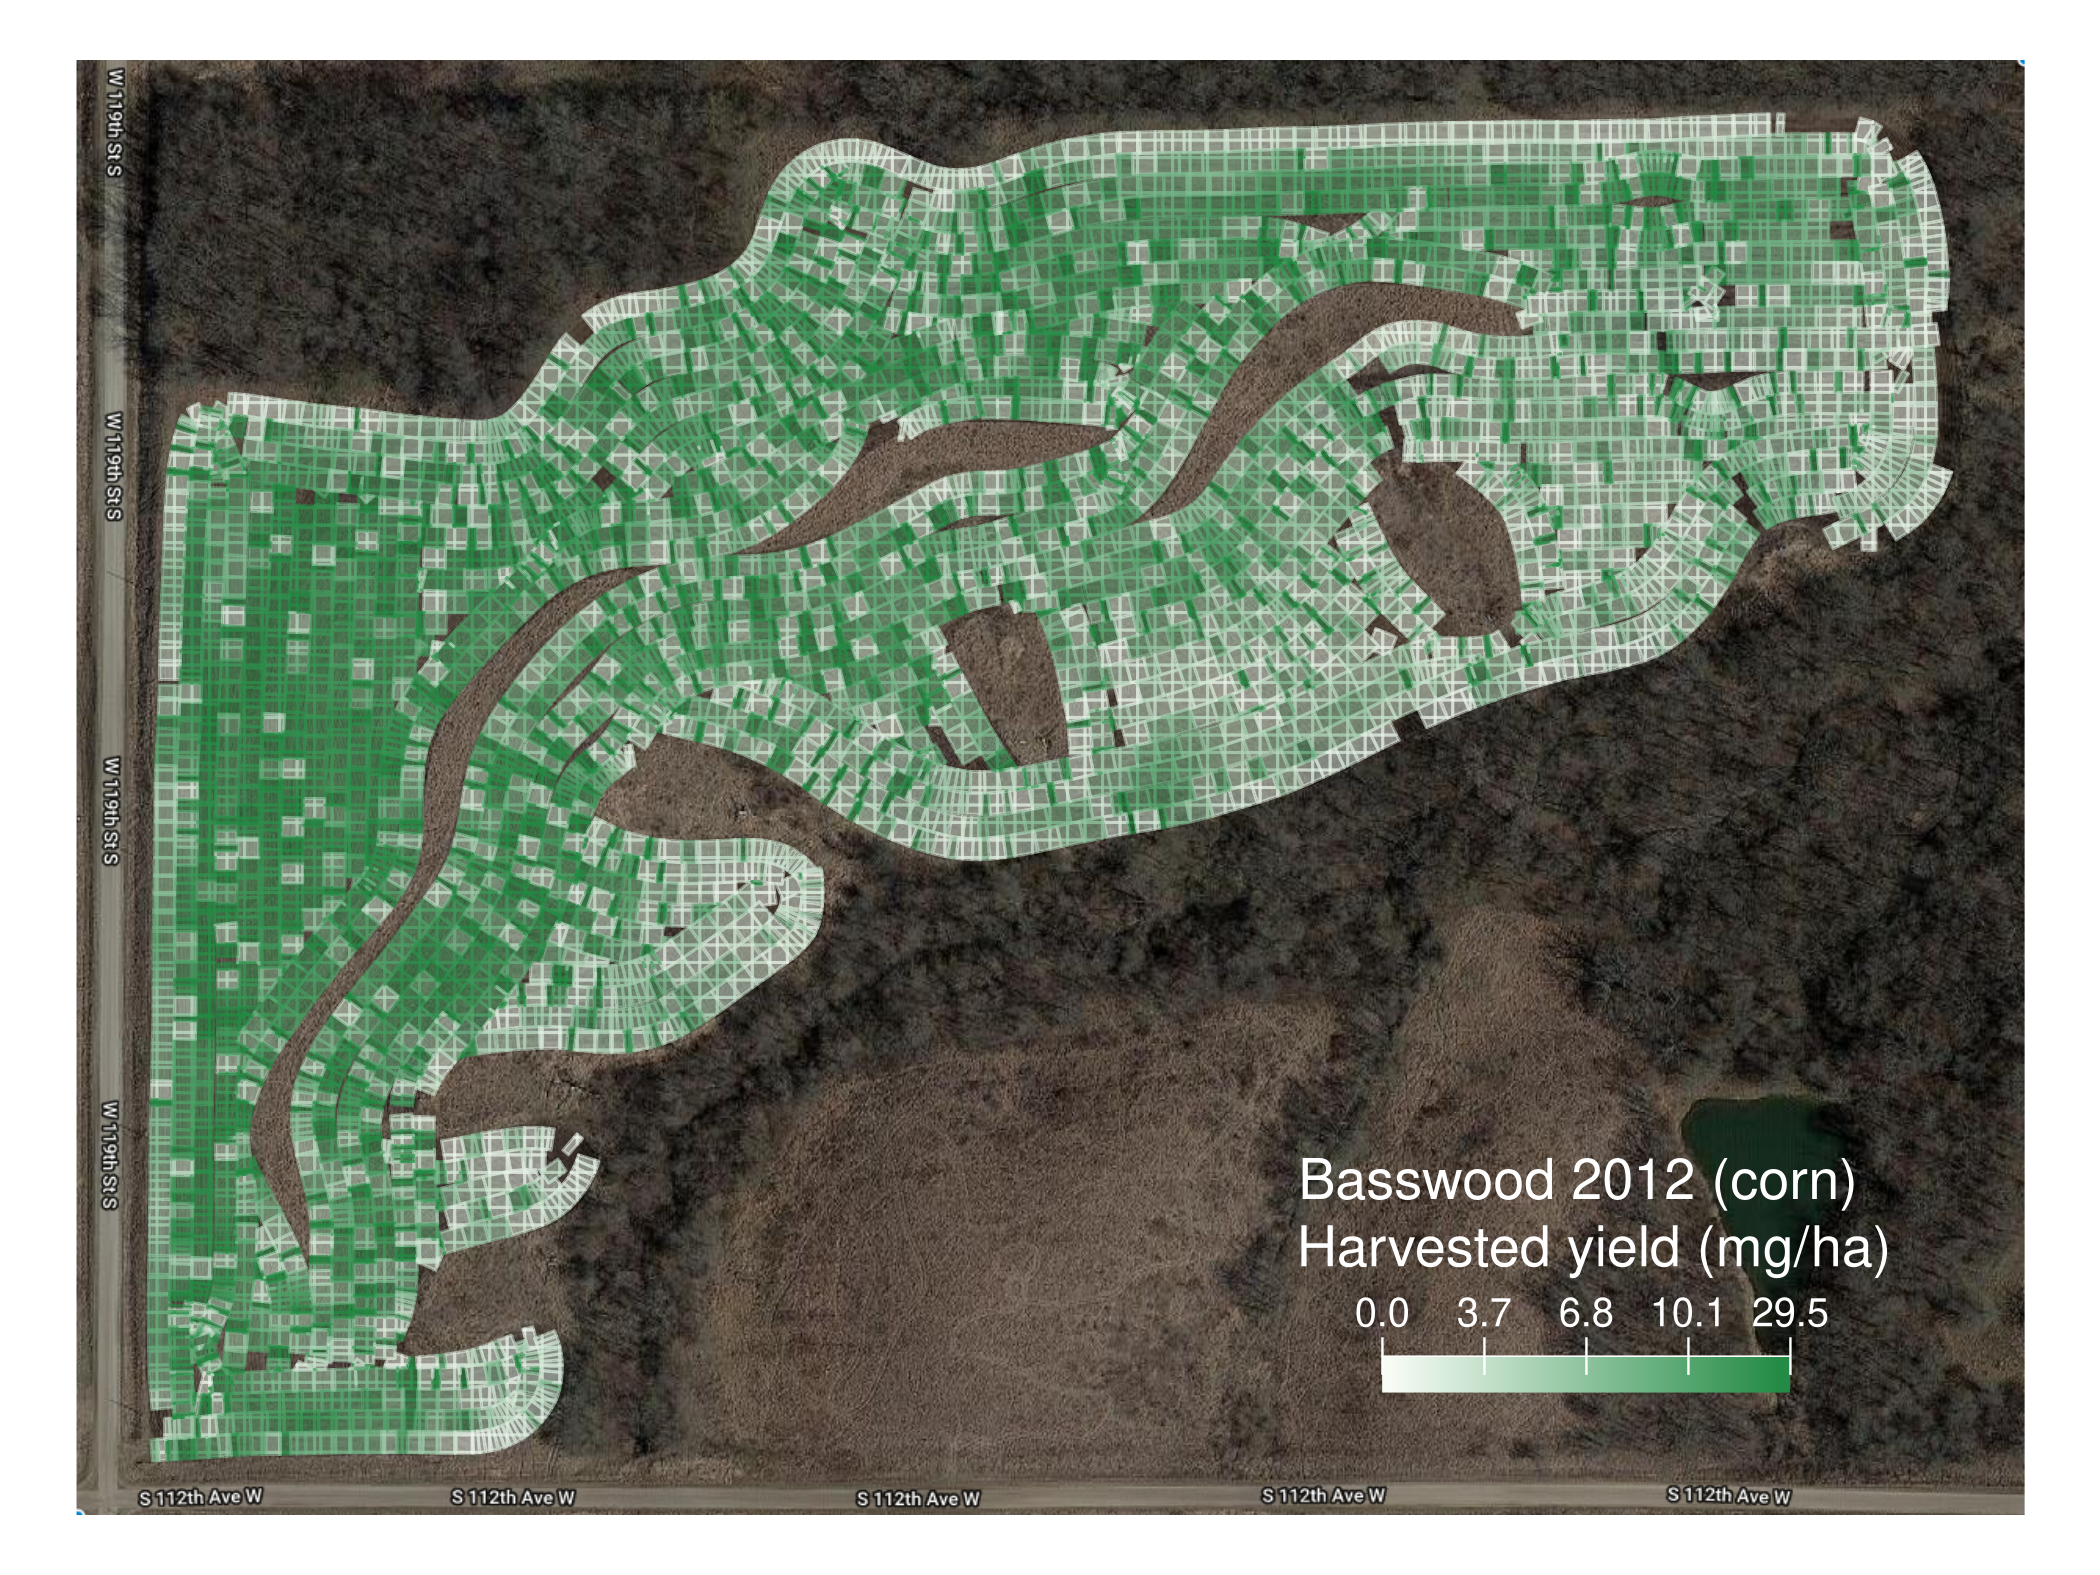
\includegraphics[width=0.95\textwidth]{./figures/maps/basswood_2012_04_chopped_res5_5.png}}
    \only<5>{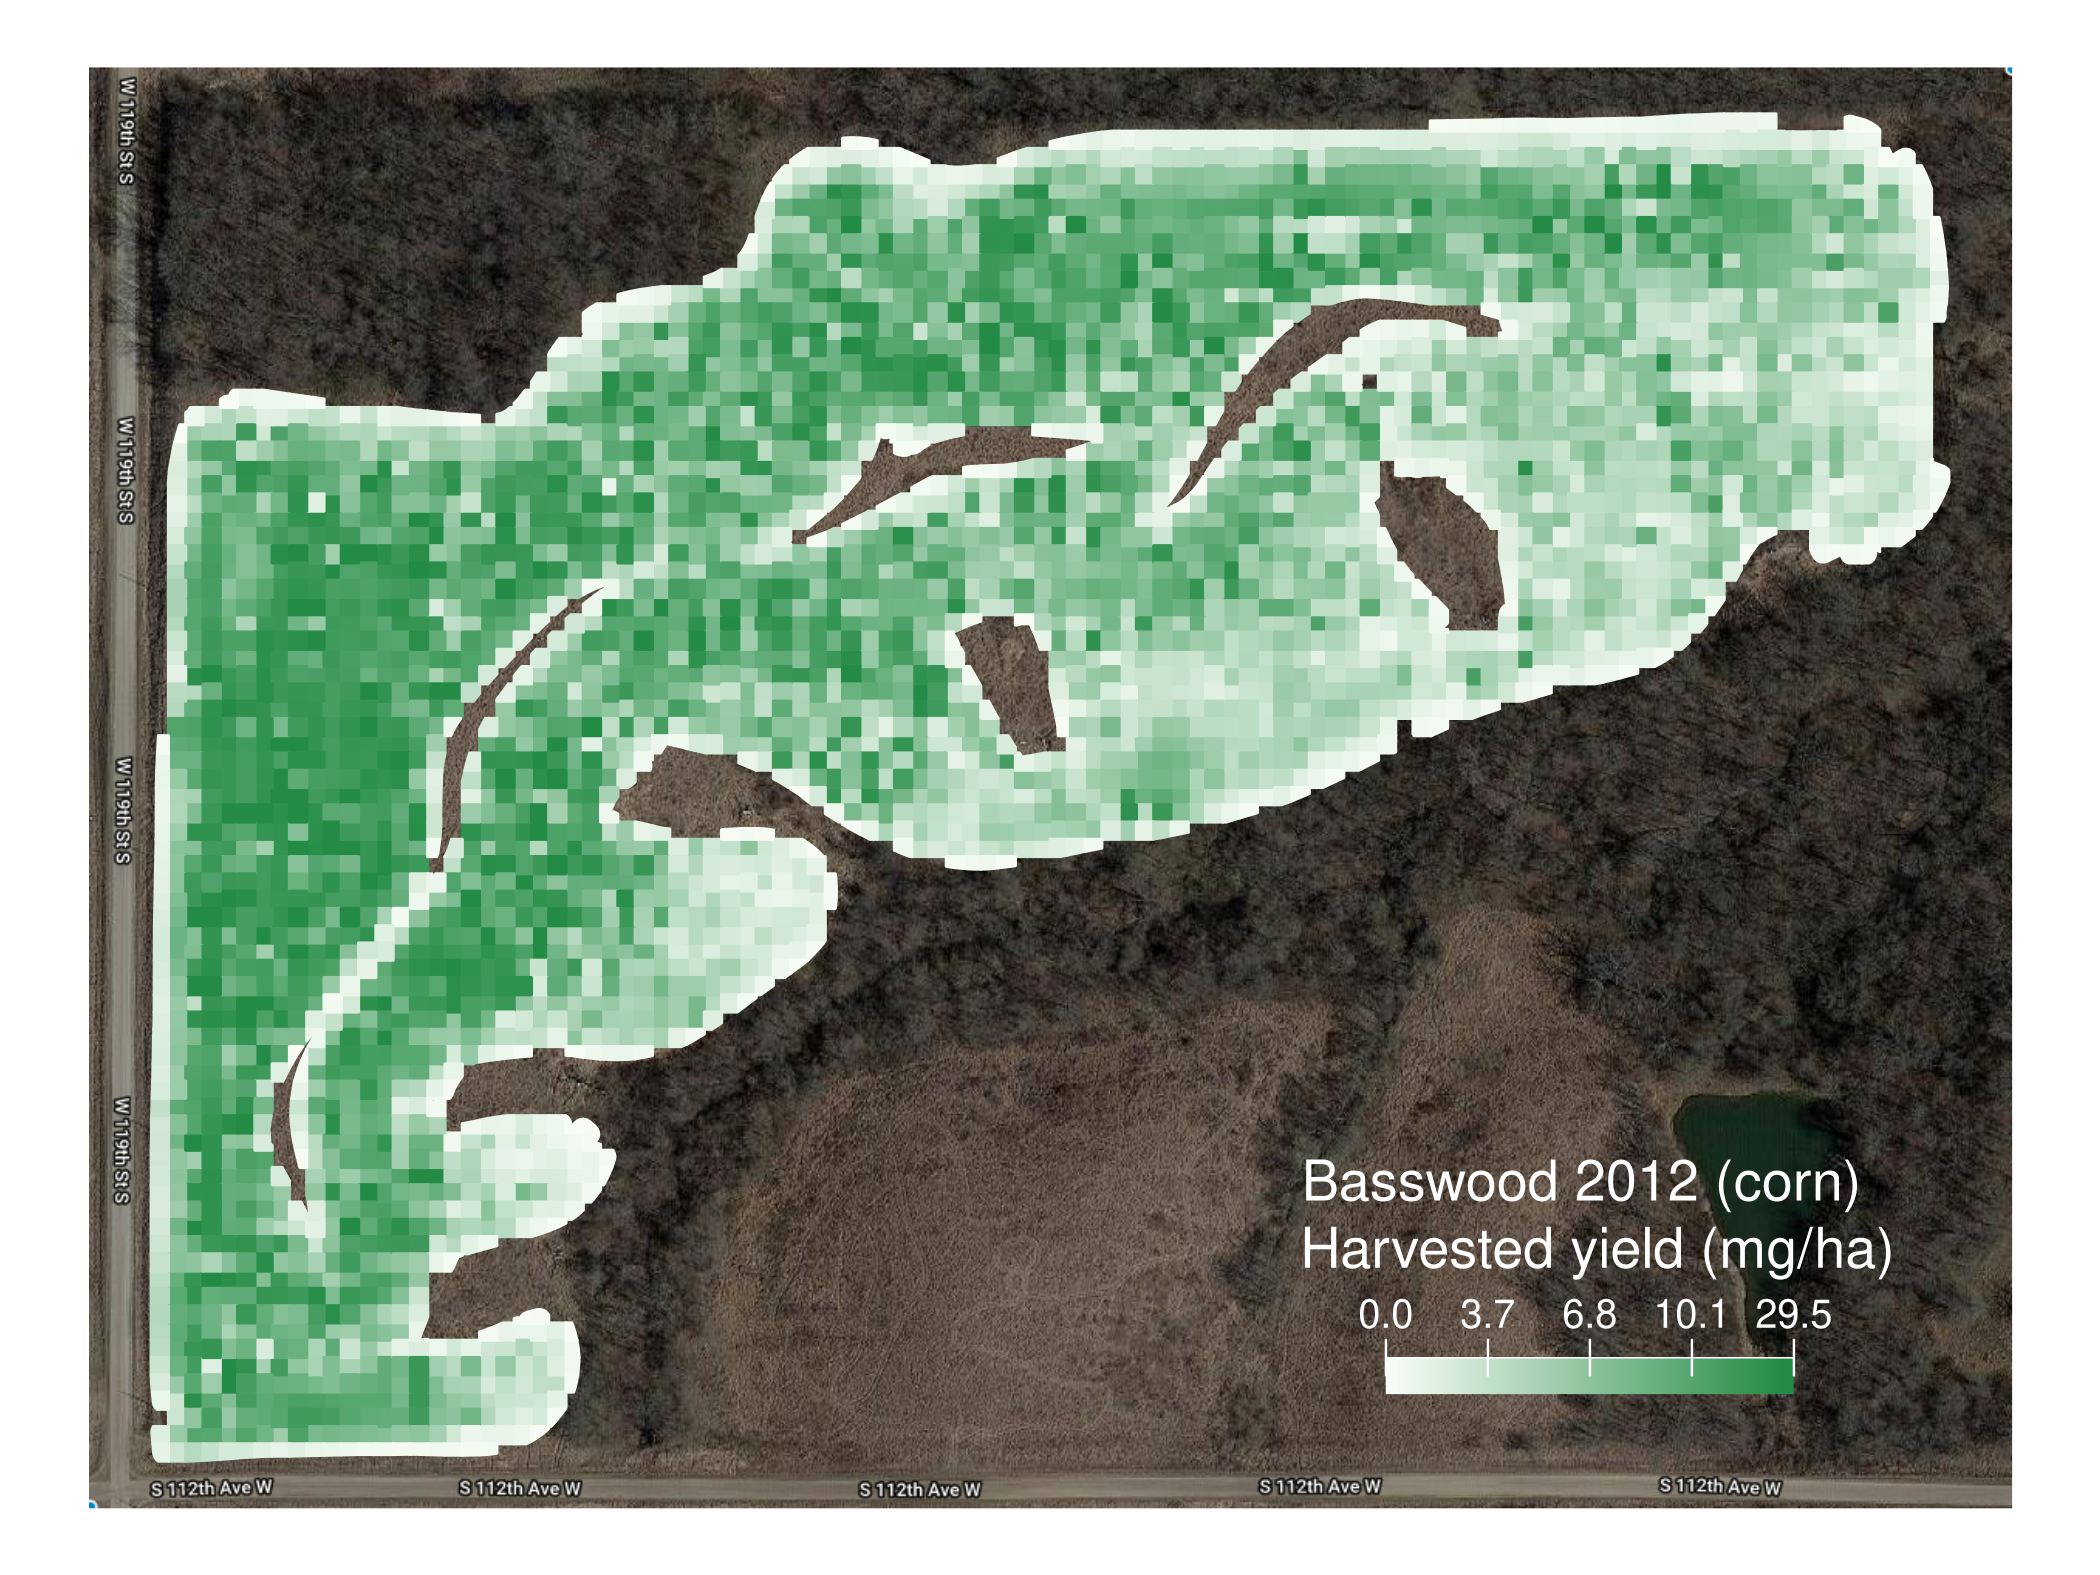
\includegraphics[width=0.95\textwidth]{./figures/maps/basswood_2012_05_apportioned_res5_5.png}}
    \only<6>{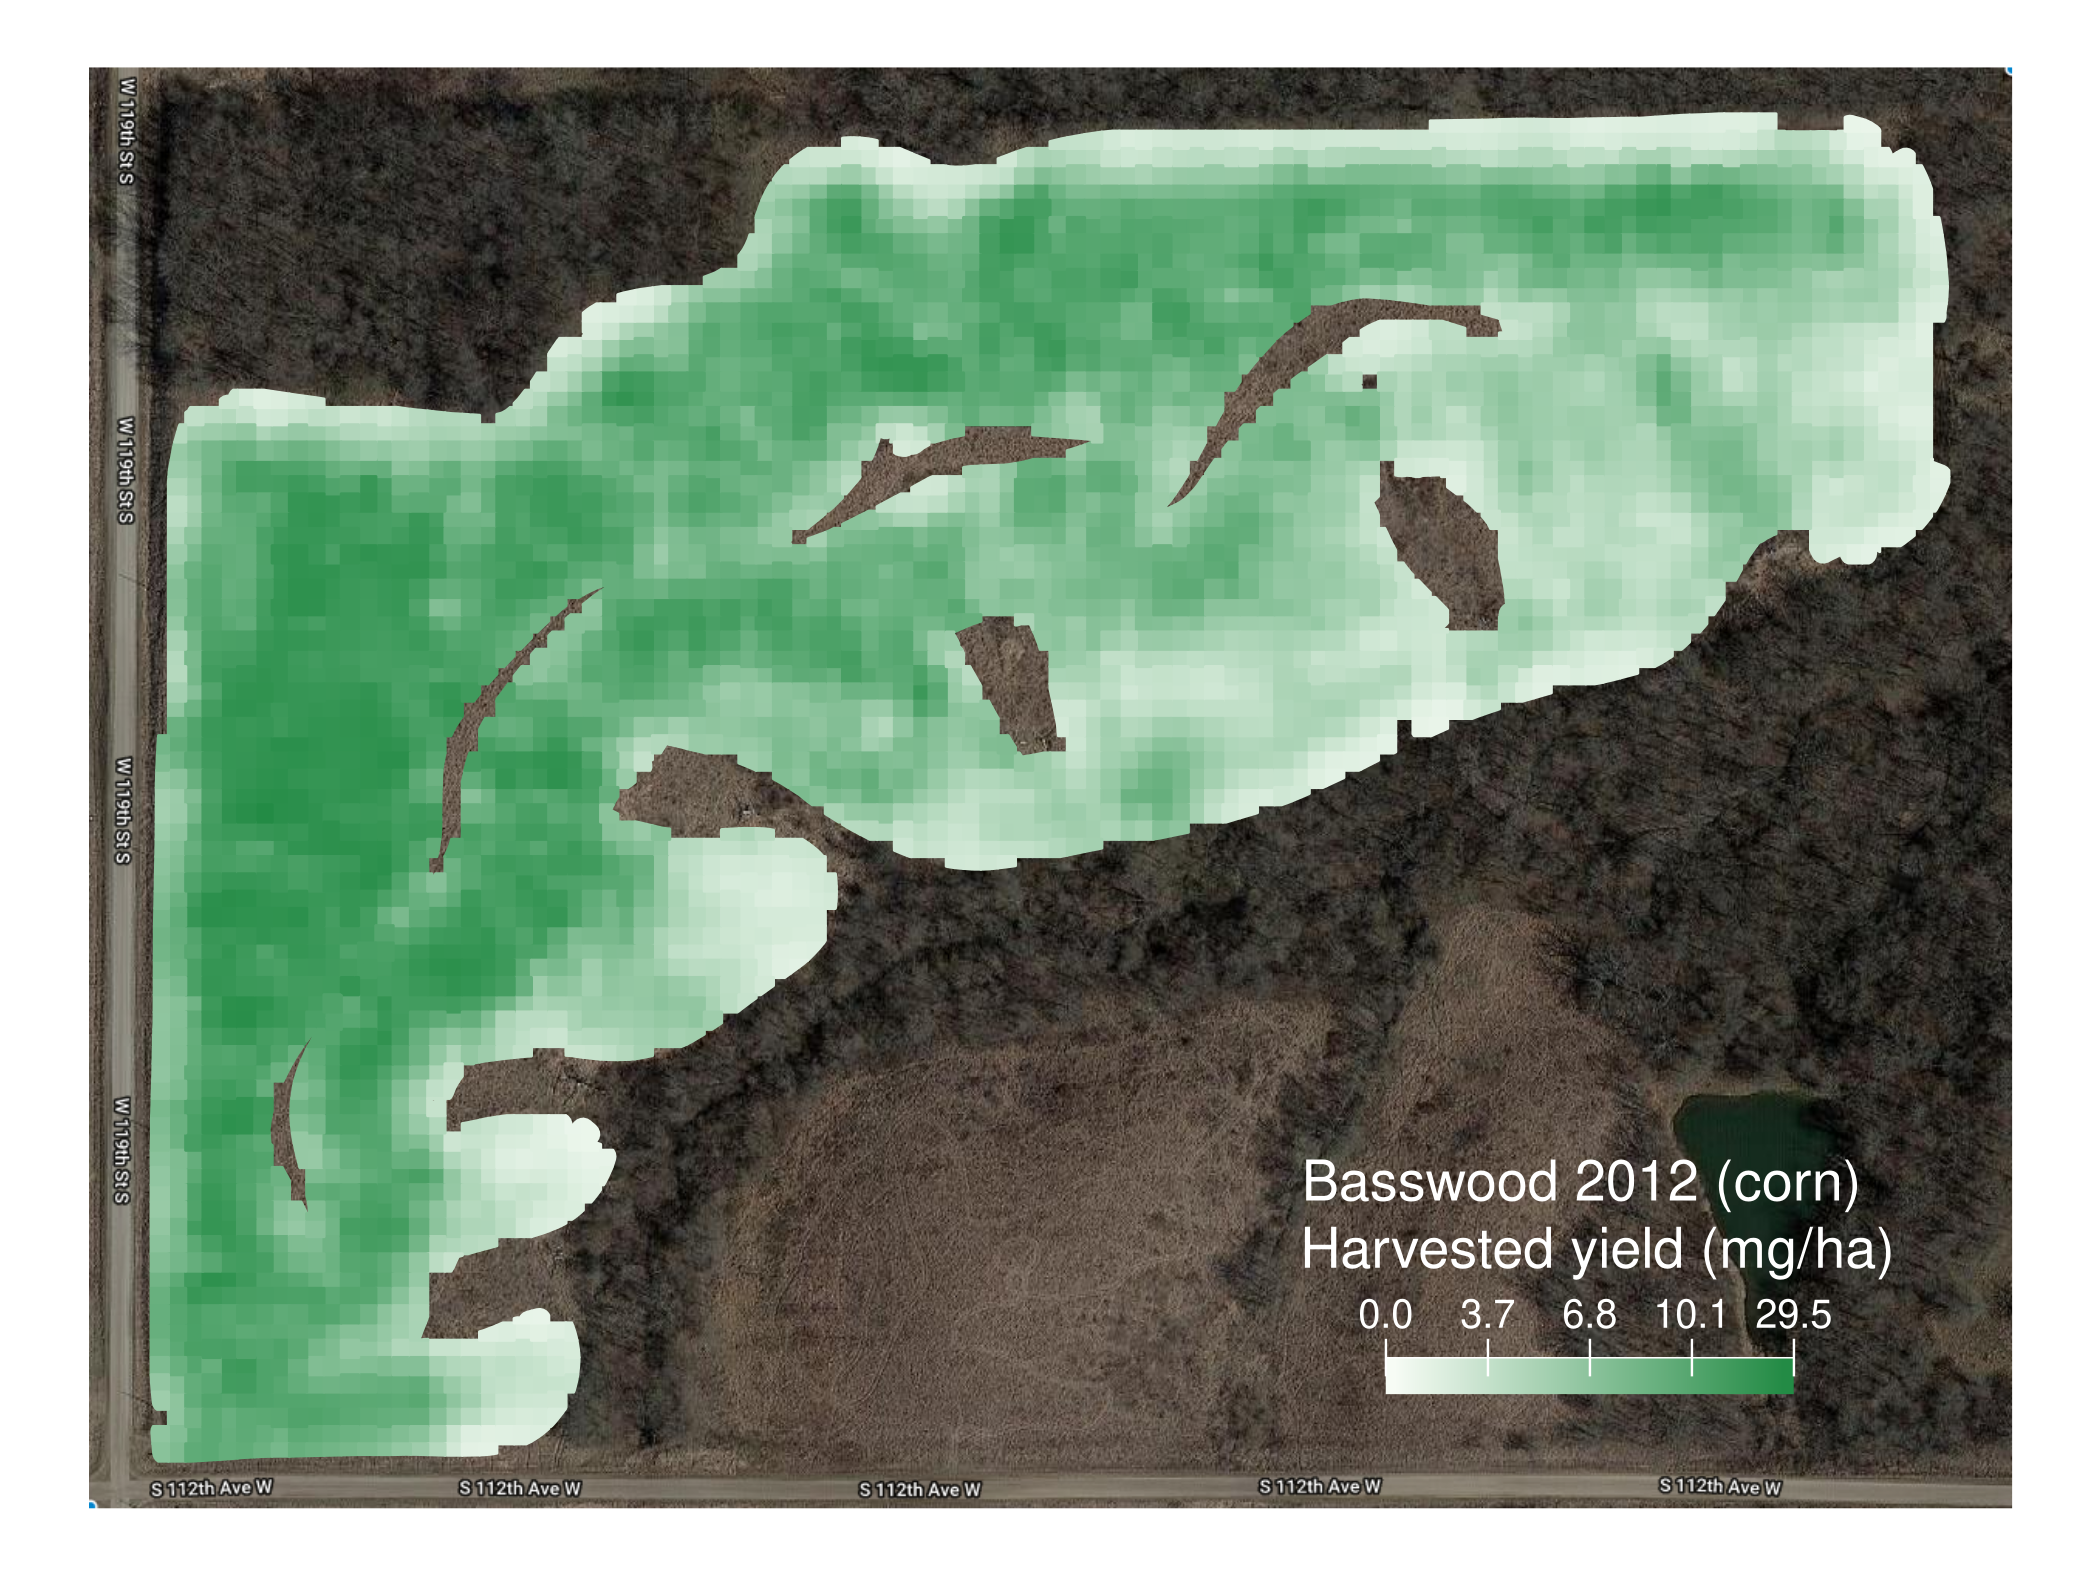
\includegraphics[width=0.95\textwidth]{./figures/maps/basswood_2012_06_smoothed_res5_5.png}}
  \end{center}
\end{frame}

%%%%%%%%%%%%%%%%%%%%%%%%%%%%%%%%%%%%%%%%%%%%%%%%%%%%%%%%%%%%%%%%%%%%%%%%%%
% Discussion                                                             %
%%%%%%%%%%%%%%%%%%%%%%%%%%%%%%%%%%%%%%%%%%%%%%%%%%%%%%%%%%%%%%%%%%%%%%%%%%

\section{Discussion}

\begin{frame}[t]
  \frametitle{The YAYs!}

  % Compare with other work

  \begin{itemize}
    \item<2-> Constructive approach motivated by data acquisition
      dynamics.
    \item<3-> Modeling mass to partially work around some of the
      uncertainty propagation channels.
    \item<4-> Autonomous: no user-defined thresholds for automatic
      processing and more consistent results across data sets.
    \item<5-> No observations were harmed during the making of this film.
    \item<6-> Apportioned observations are aligned for spatio-temporal
      analysis (spatial registration).
  \end{itemize}
  
\end{frame}

\begin{frame}[t]
  \frametitle{The not-so-YAYs!}

  % Compare with other work

  \begin{itemize}
    \item<2-> Smoothing is $O(N^3)$, but many approximations are
      readily available.
    \item<3-> Tessellation, if improved naively, involves $(N-1)!$ operations.
    \item<4-> Time lag processing rules sold separately.
  \end{itemize}
  
\end{frame}

%%%%%%%%%%%%%%%%%%%%%%%%%%%%%%%%%%%%%%%%%%%%%%%%%%%%%%%%%%%%%%%%%%%%%%%%%%
% Future work                                                            %
%%%%%%%%%%%%%%%%%%%%%%%%%%%%%%%%%%%%%%%%%%%%%%%%%%%%%%%%%%%%%%%%%%%%%%%%%%

\section{Future work}

\begin{frame}
  \frametitle{Variability quantification}

  % How to quantify the smoothness.
  % How challenging is my dataset?
  % Show two rectangle plots

  \begin{figure}
    %\includegraphics[width=0.80\textwidth]{./figures/maps/basswood_2007_07_gallery_res5_5.png}
    %\includegraphics[width=0.80\textwidth]{./figures/maps/basswood_2009_07_gallery_res5_5.png}

    \caption{Apportioned (left) and smoothed (right) maps for two
      datasets with an apparent difference in variability.}
  \end{figure}
  
\end{frame}

\begin{frame}
  \frametitle{Improvement quantification}

  % How to quantify the improvement in terms of ``variance reduction''
  % What's behind the fancy plots?
  \begin{figure}
    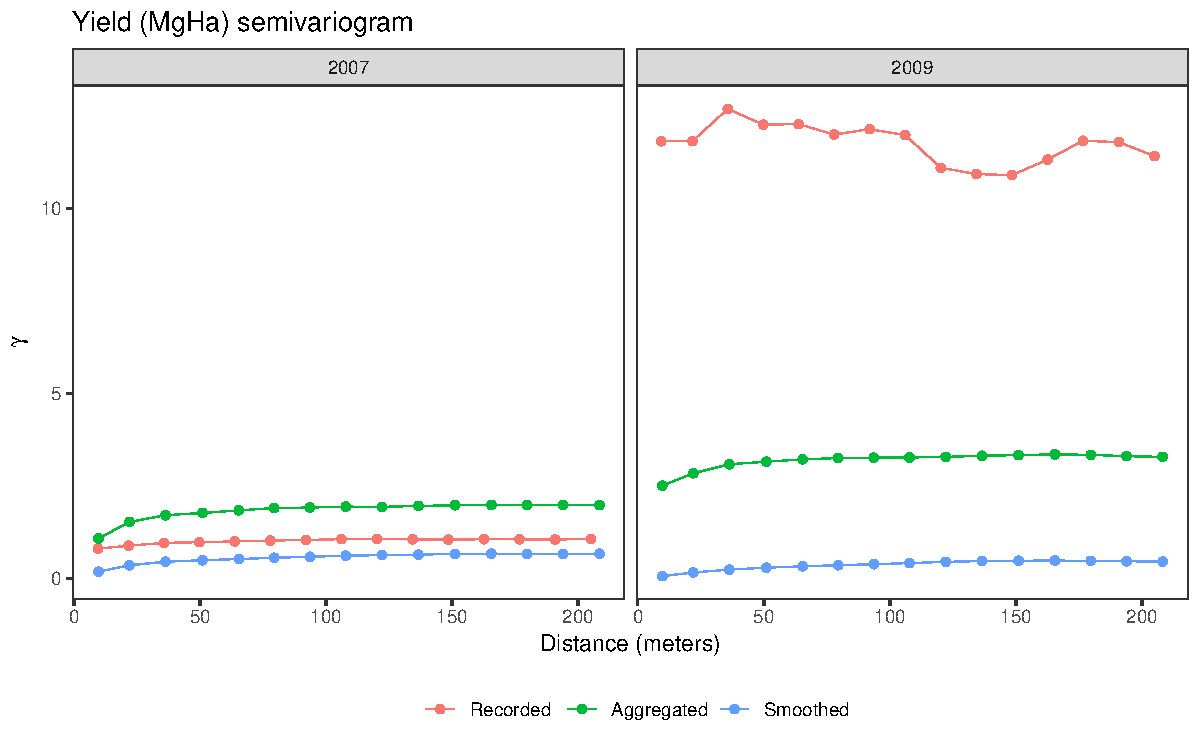
\includegraphics[width=0.95\textwidth]{./figures/semivariogram.pdf}
    \caption{Semivariogram of the yield monitor data}
  \end{figure}

\end{frame}

\begin{frame}
  \frametitle{Resolution selection}
  
  \begin{figure}
    %\includegraphics[width=0.4\textwidth]{./figures/maps/basswood_2012_06_smoothed_res9_9.png}
    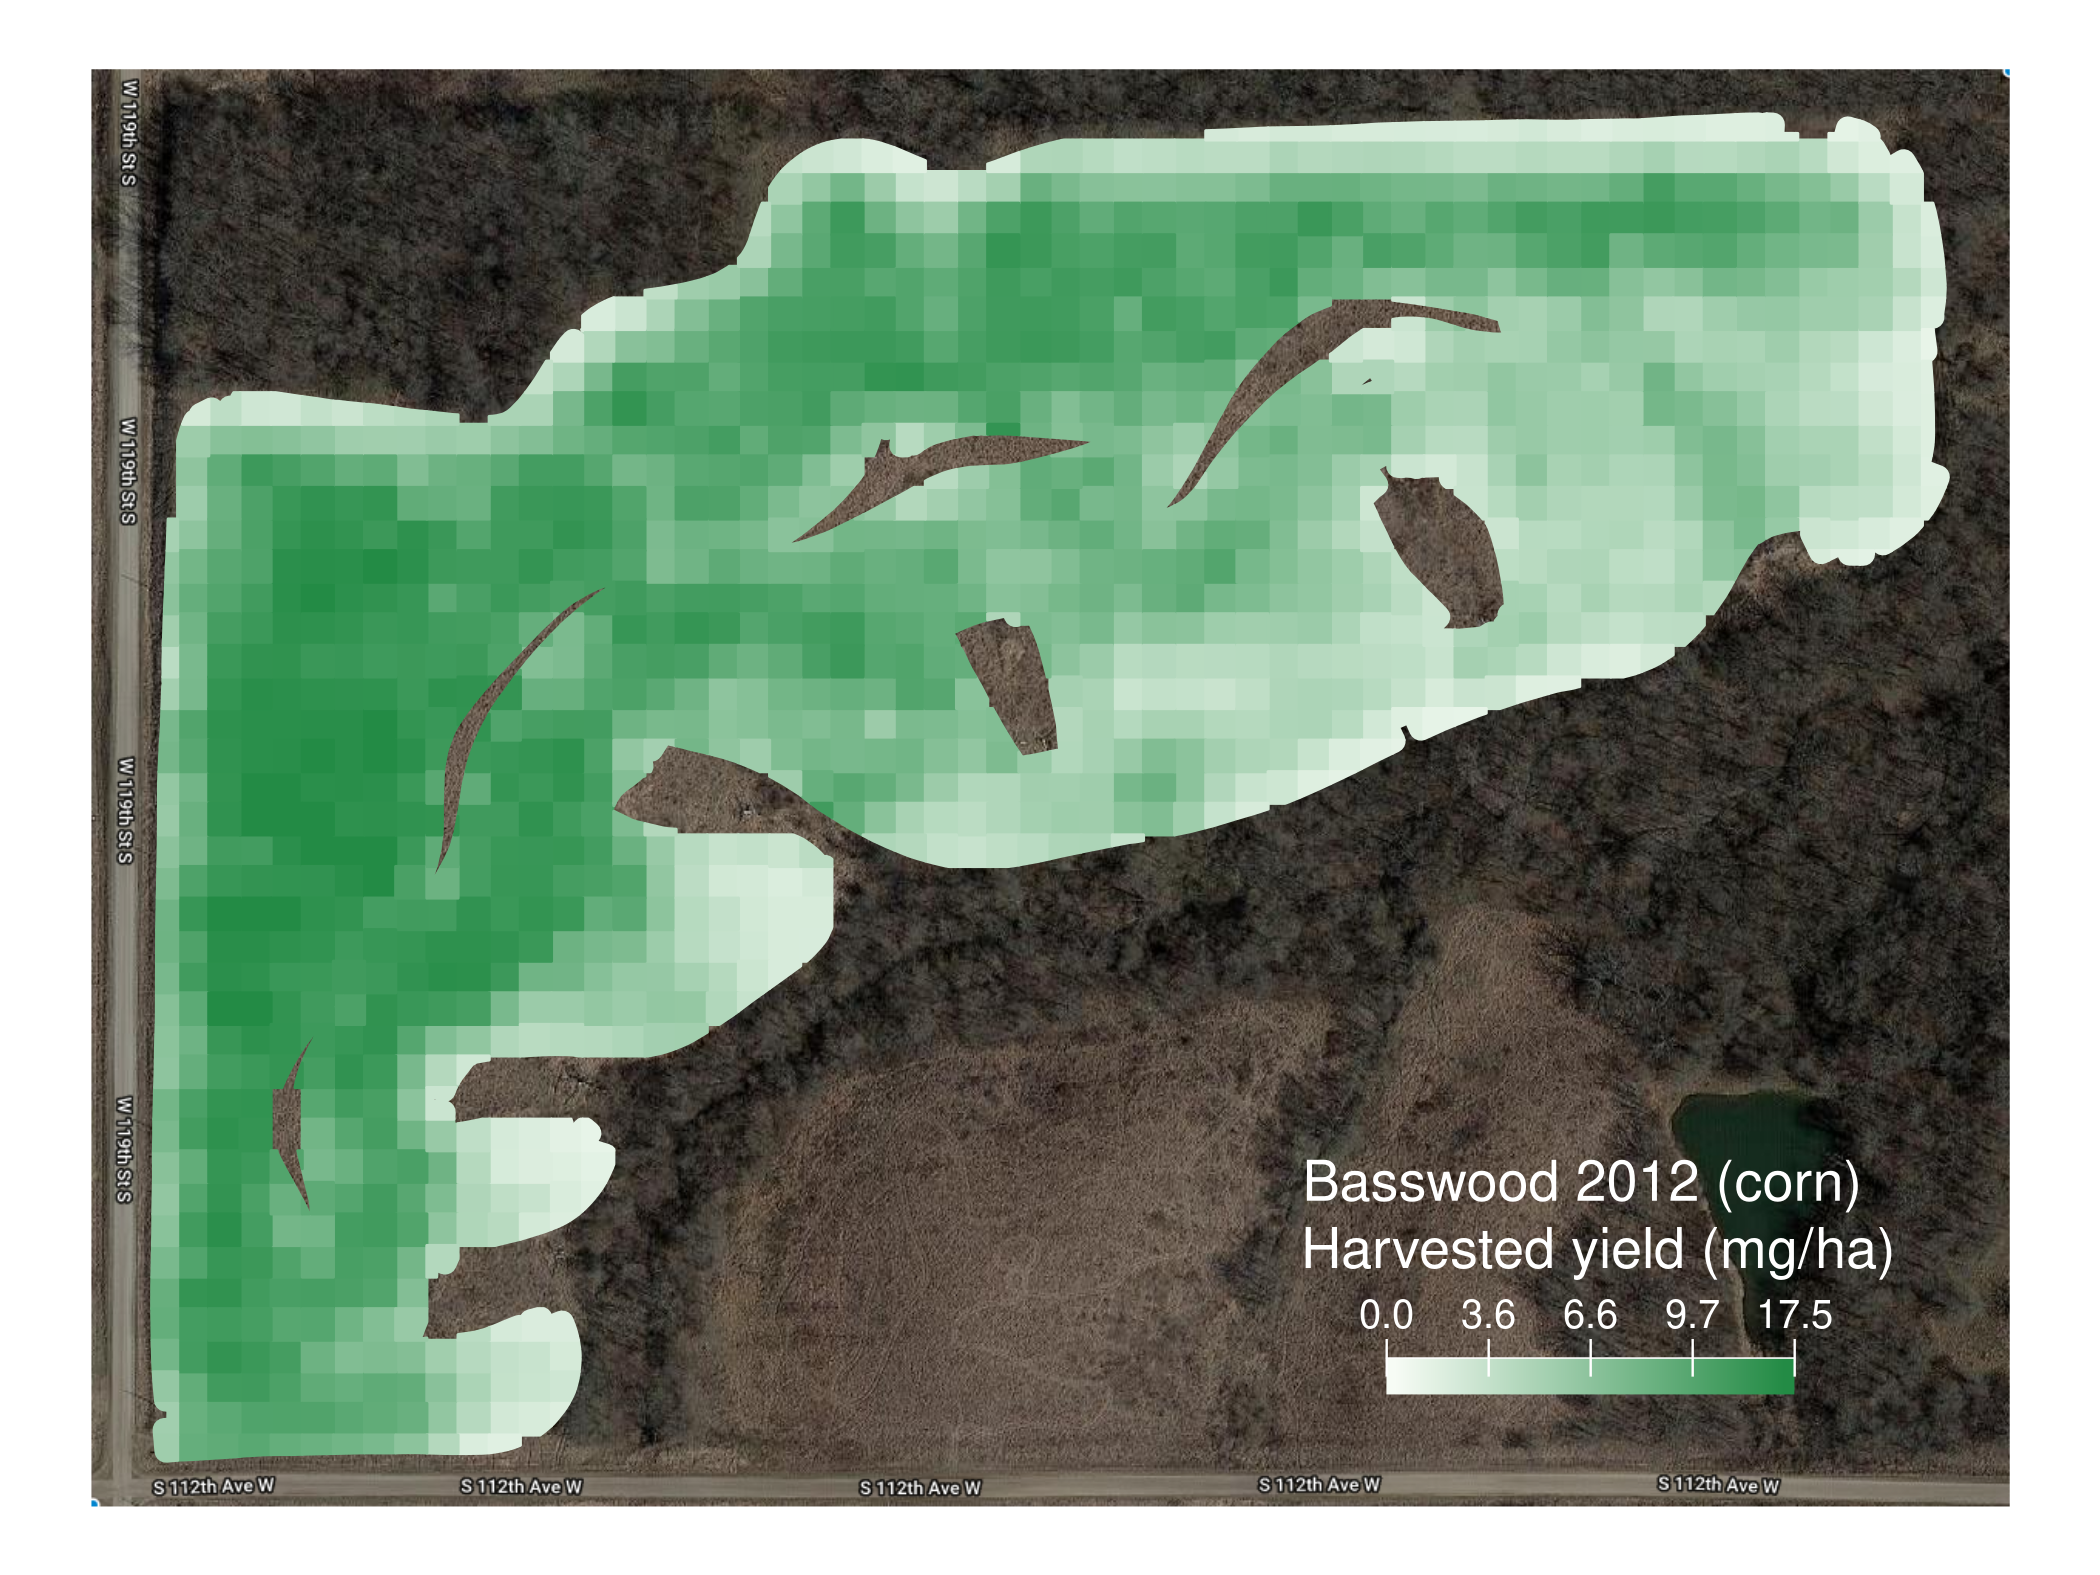
\includegraphics[width=0.4\textwidth]{./figures/maps/basswood_2012_06_smoothed_res7_7.png}

    \vspace{0px}
    
    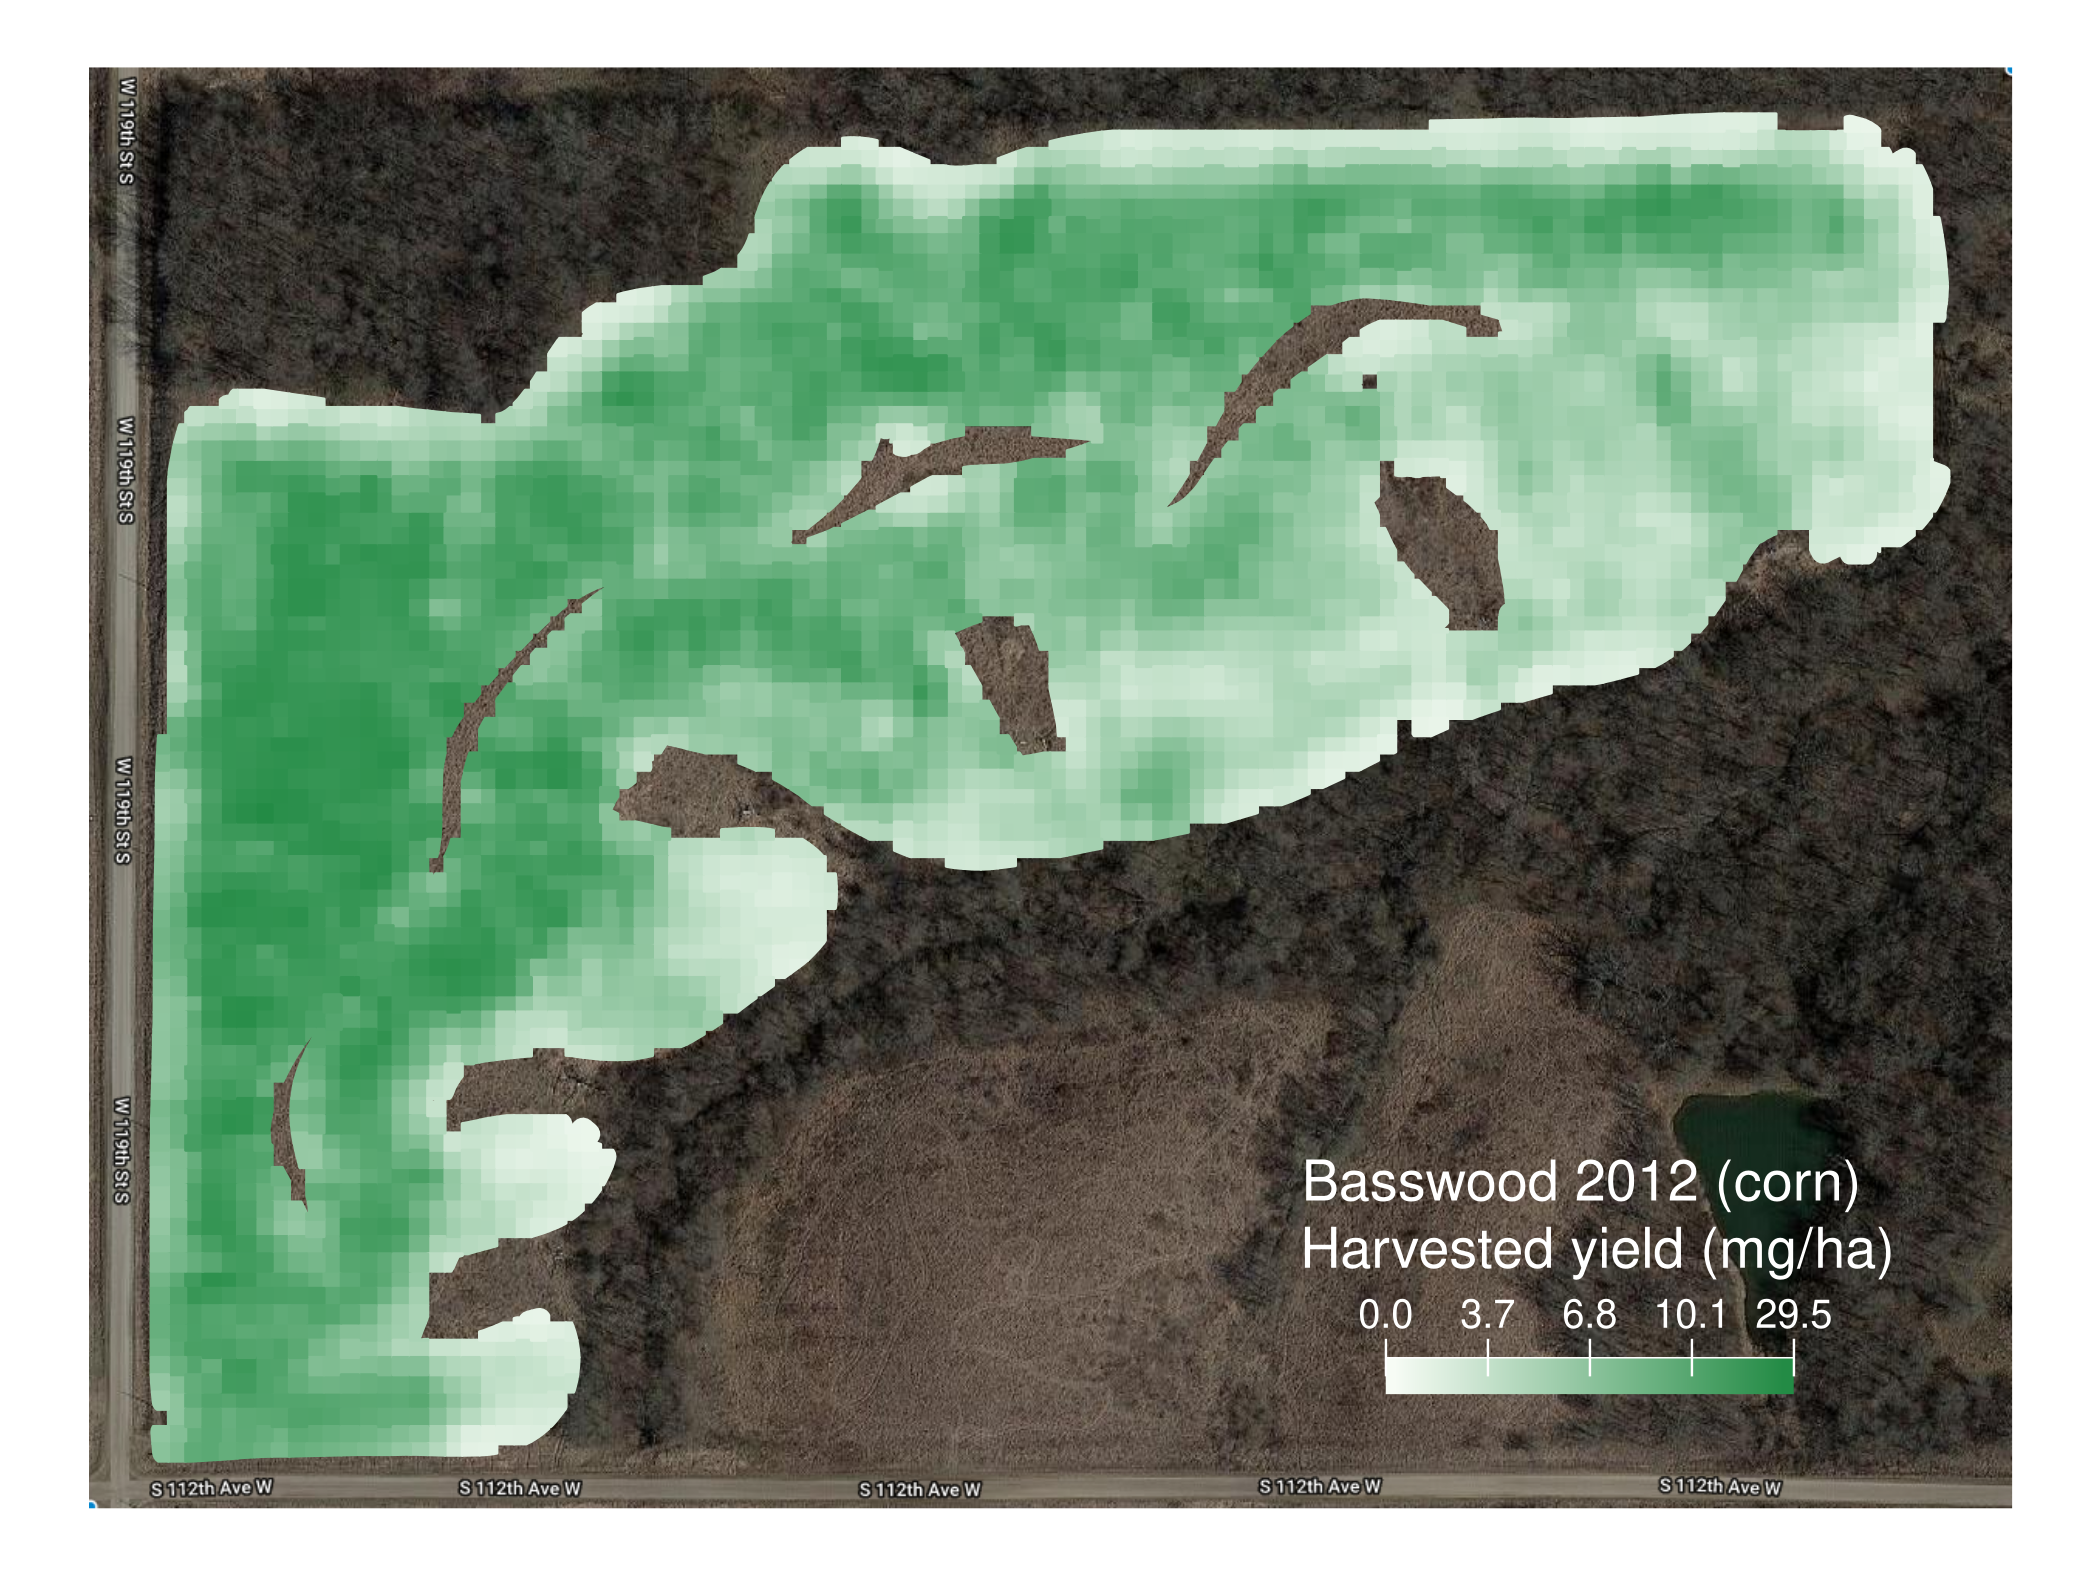
\includegraphics[width=0.4\textwidth]{./figures/maps/basswood_2012_06_smoothed_res5_5.png}
    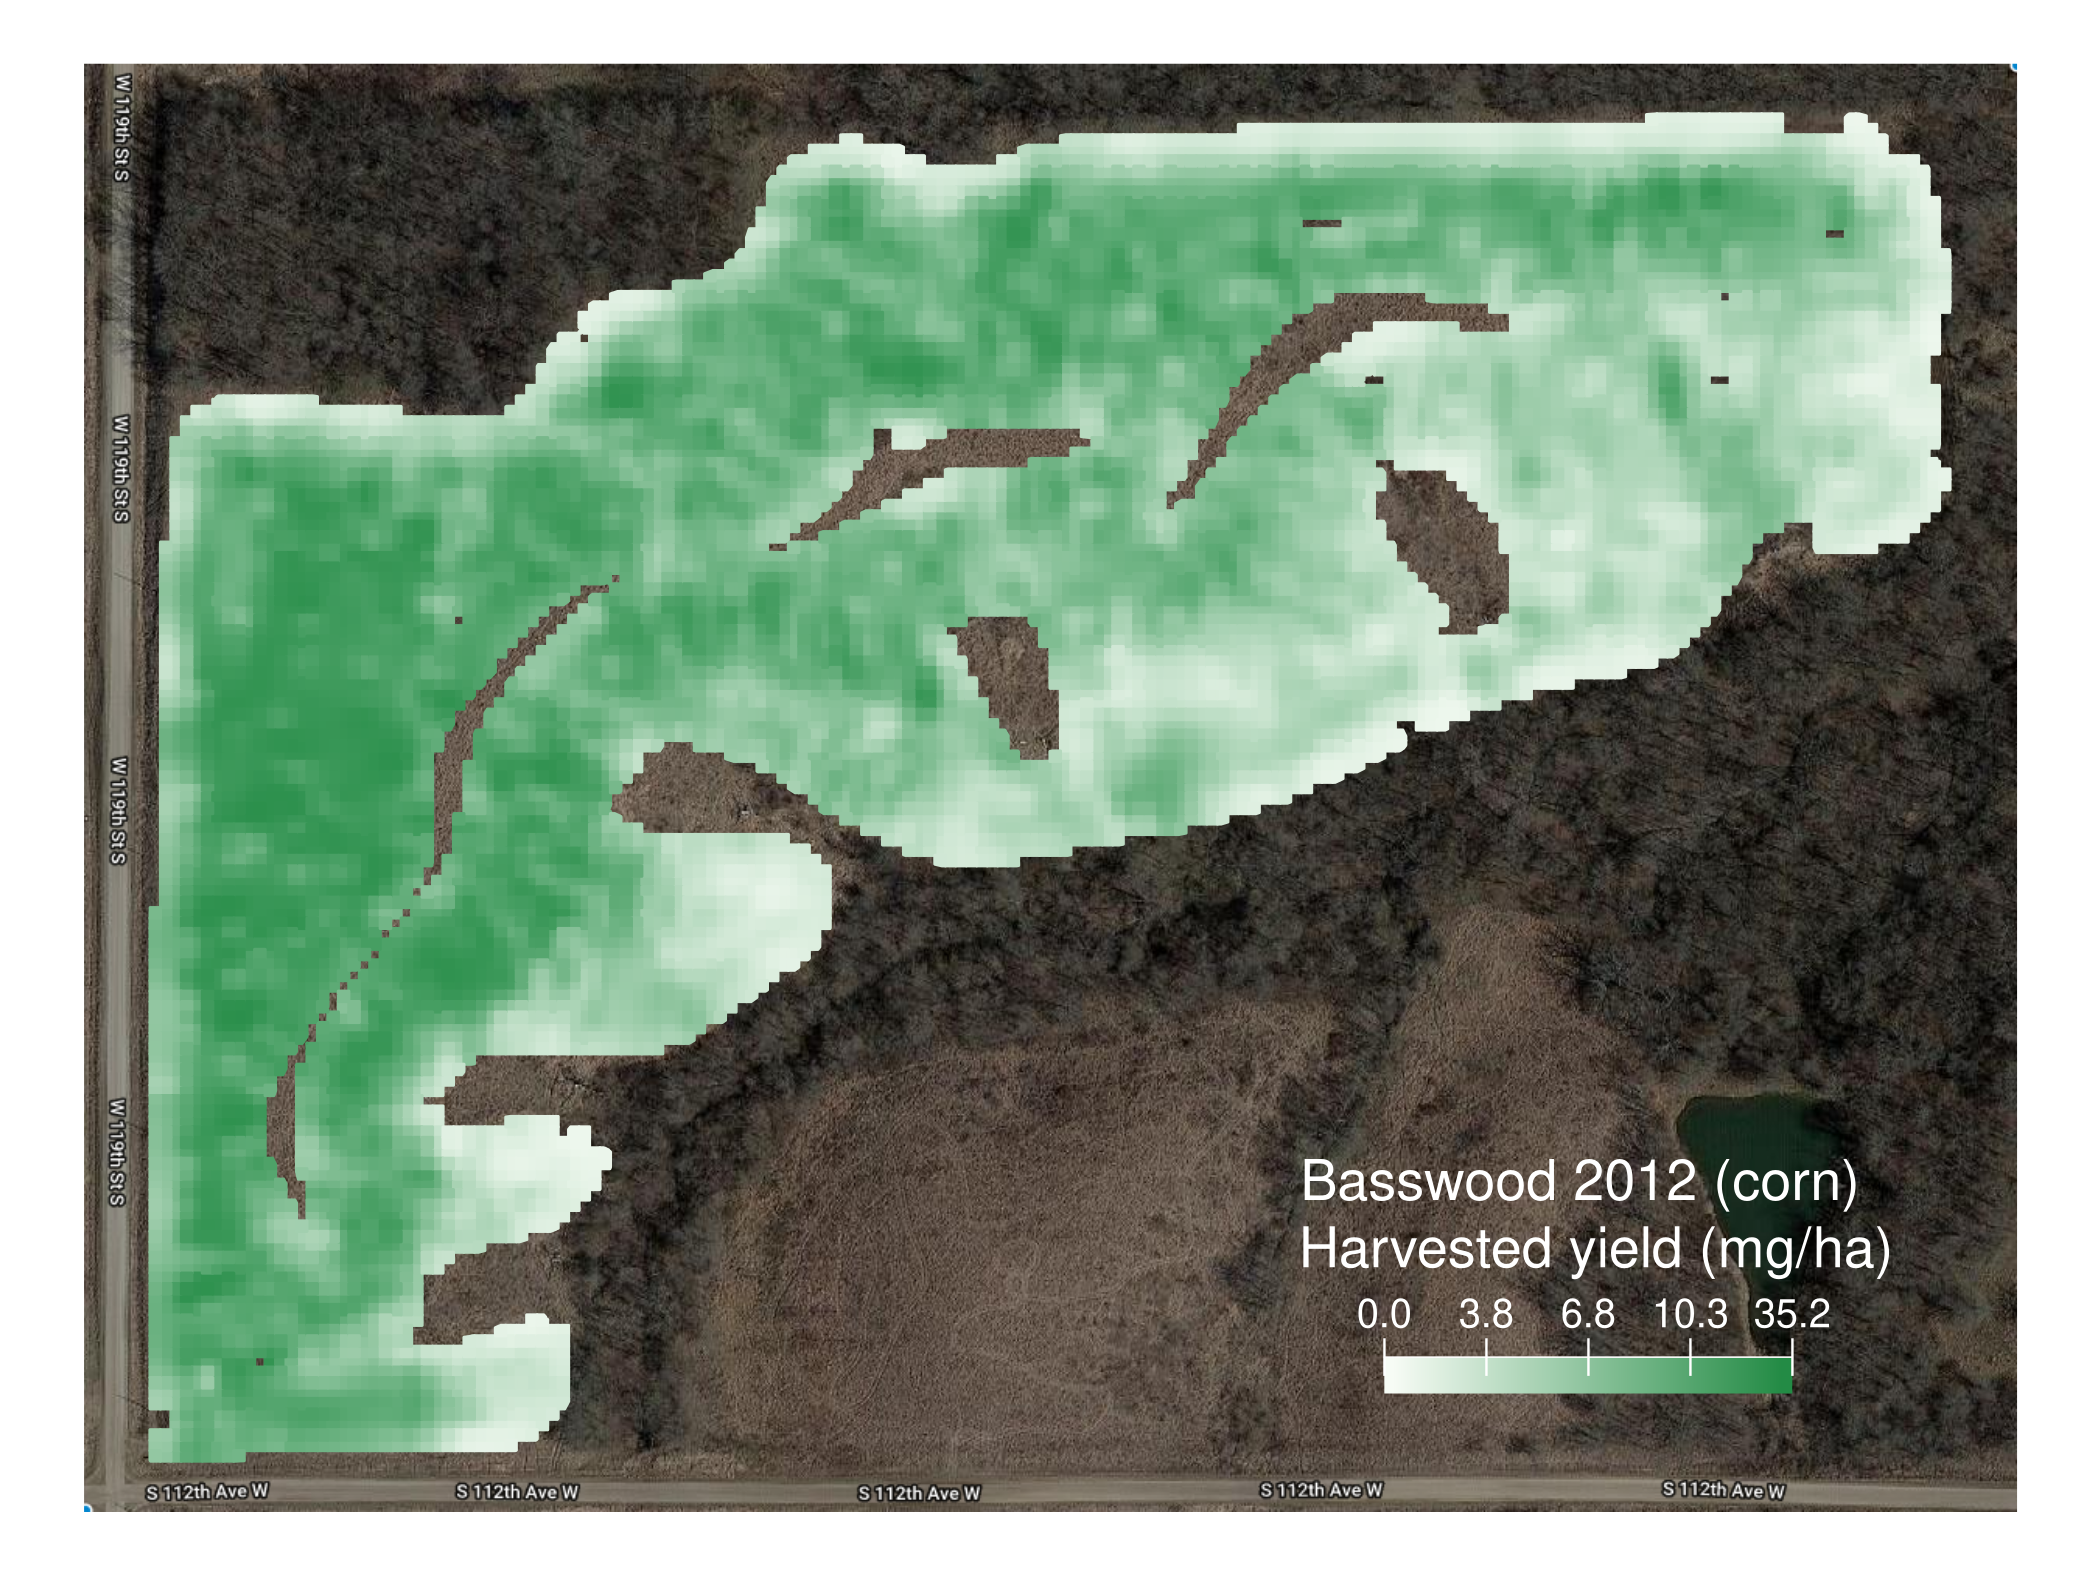
\includegraphics[width=0.4\textwidth]{./figures/maps/basswood_2012_06_smoothed_res3_3.png}

    \caption{Smoothed map at four different resolutions. Top: 9m, 7m;
      bottom: 5m, 3m.}

  \end{figure}
  
  % Show maps at different resolutions: aggregate, 10, 7, 5,
  % 3. Overfits?
  % Resolution selection
  % Why does the map deteriorate?
  
\end{frame}

%%%%%%%%%%%%%%%%%%%%%%%%%%%%%%%%%%%%%%%%%%%%%%%%%%%%%%%%%%%%%%%%%%%%%%%%%%
% References                                                             %
%%%%%%%%%%%%%%%%%%%%%%%%%%%%%%%%%%%%%%%%%%%%%%%%%%%%%%%%%%%%%%%%%%%%%%%%%%

\section*{References}

\begin{frame}[allowframebreaks]
  \frametitle{References}

  See Creative Component writing.

  % \scriptsize
  % \nocite{*}

  % \bibliography{../writing/reference/references.bib}
  % \bibliographystyle{plainnat}
\end{frame}

\end{document}
%%% Local Variables:
%%% mode: latex
%%% TeX-master: t
%%% End:
